\documentclass[sigconf, review, anonymous]{acmart}

%% Rights management information. Placeholder values for double-blind
%% review submission; will be replaced from the rights confirmation
%% email for camera-ready.
\setcopyright{acmlicensed}
\copyrightyear{2026}
\acmYear{2026}
\acmDOI{XXXXXXX.XXXXXXX}
\acmConference[SIGSPATIAL '26]{34th ACM International Conference on
  Advances in Geographic Information Systems}{November 3--6,
  2026}{Riverside, CA, USA}
\acmISBN{978-1-4503-XXXX-X/2026/11}

\usepackage{amsmath, amsthm}
\let\Bbbk\relax
\usepackage{amssymb}
\usepackage{enumitem}
\usepackage{float}
\usepackage[capitalise]{cleveref}
\usepackage{tikz}
\usepackage{xcolor}
\usepackage[normalem]{ulem}
\usepackage{multirow}
\usepackage{subcaption}
\usepackage{booktabs}
\usepackage{makecell}

% Cross-week noise scale; defined once so future renaming touches only this line.
\newcommand{\NF}{\tau}
\newcommand{\NFG}{\tau_{\textsf{global}}}

% Inline annotation macros: \hamid{...} prepends "HAMID:" in blue,
% \jeff{...} prepends "JEFF:" in red.
% Remove or redefine to identity before camera-ready.
\newcommand{\hamid}[1]{{\color{blue}\textbf{HAMID:}\ #1}}
\newcommand{\jeff}[1]{{\color{red}\textbf{JEFF:}\ #1}}

\begin{document}

\title{A Markov Chain Pipeline for Link-Level Urban Traffic}

\author{Anonymous}
\affiliation{%
  \institution{Anonymous}
  \country{Anonymous}
}
\email{anonymous@example.org}

\renewcommand{\shortauthors}{Anonymous}

\begin{abstract}
We fit calibrated Markov chains to urban traffic on a
$99{,}716$-link metropolitan road network using $30$~days of
probe GPS. Raw GPS fixes are projected onto the network with
the hidden Markov map-matcher of Newson and
Krumm~\cite{newson2009hmm}, run through the Leuven Map-Matching
library~\cite{meert2018hmm,leuvenmapmatching}; accumulated into
a sparse popularity matrix
$C \in \mathbb{Z}_{\ge 0}^{T \times N}$ with $T = 8{,}640$
five-minute bins; and smoothed by one step of graph
diffusion~\cite{shuman2013gsp} at a strength calibrated to the
empirical cross-week noise floor of the corpus. The smoothed
prior drives a Markov chain on the road graph whose parameters
are fit from the corpus rather than chosen by hand: a damping
rate from the empirical trip-length distribution, and
road-type transition weights (speed limit, lane count) from
gradient descent. On an $840$-bin evaluation sample
($120$ random bins per day of the week), the road-type
calibration reduces the chain's mean per-link relative error
against a uniform-transition baseline.
\end{abstract}

%% CCS concepts. Placeholders; final values must be generated at
%% https://dl.acm.org/ccs and replace the entries below.
\begin{CCSXML}
<ccs2012>
  <concept>
    <concept_id>10010147.10010257.10010321</concept_id>
    <concept_desc>Computing methodologies~Modeling and simulation</concept_desc>
    <concept_significance>500</concept_significance>
  </concept>
  <concept>
    <concept_id>10002951.10003317.10003347</concept_id>
    <concept_desc>Information systems~Geographic information systems</concept_desc>
    <concept_significance>300</concept_significance>
  </concept>
  <concept>
    <concept_id>10010147.10010178.10010187</concept_id>
    <concept_desc>Computing methodologies~Spatial and physical reasoning</concept_desc>
    <concept_significance>100</concept_significance>
  </concept>
</ccs2012>
\end{CCSXML}

\ccsdesc[500]{Computing methodologies~Modeling and simulation}
\ccsdesc[300]{Information systems~Geographic information systems}
\ccsdesc[100]{Computing methodologies~Spatial and physical reasoning}

\keywords{PageRank, road traffic, GPS trajectory, map matching, hidden Markov model, graph diffusion, urban mobility, per-link traffic estimation}

\maketitle

\section{Introduction}

Estimating how vehicle traffic distributes across the individual
road links of a metropolitan area is a basic input for routing,
control, and incident analysis. Doing it at the resolution of
\emph{every link} from probe GPS alone is harder than it looks:
coverage is sparse and uneven, the network has tens of thousands
of edges, and most per-bin per-link cells contain no observations
at all. We study the problem on a $99{,}716$-link road network of
Salt Lake City using $30$ days of probe trajectories.

The approach is a Markov chain on the road graph driven by a
per-link prior $E_b \in \mathbb{R}^N$ assembled end-to-end from
the raw data: GPS fixes are projected onto the network with the
hidden Markov matcher of Newson and Krumm~\cite{newson2009hmm}
(in the Leuven
implementation~\cite{meert2018hmm,leuvenmapmatching} that we run),
aggregated into a sparse popularity matrix
$C \in \mathbb{Z}_{\ge 0}^{T \times N}$ over $5$-minute bins, and
smoothed by graph diffusion~\cite{shuman2013gsp} at a strength
fit from the empirical cross-week noise floor of the corpus. The
chain's damping rate and road-type transition weights (speed
limit, lane count) are fit from the corpus rather than chosen by
hand. The following sections cover these steps in order, define
the chain, and report its evaluation.

\section{Related work}
\label{sec:related-work}

The question this paper addresses is whether one can fit a
calibrated model of vehicle traffic at the resolution of
\emph{every single road link} of an entire city
($\sim 100{,}000$ links), using probe trajectories on a fixed
road network, and validate the fit against held-out weeks and
a held-out real-world intervention. The closest prior work
falls into three groups: agent-based traffic simulators that
take demand as an input rather than fit it from
data~\cite{horni2016matsim, balmer2006matsim};
origin-destination estimators that operate at a coarser zone
or node resolution~\cite{iqbal2014odmatrices, yang2017odprobe};
and PageRank-style random walks applied to urban networks for
centrality or coarse congestion
prediction~\cite{agryzkov2023nonlocal, wang2017pagerank, jiang2009ranking}.

\paragraph{MATSim and agent-based traffic simulation.}
The closest comparable effort in scope is
MATSim~\cite{horni2016matsim, balmer2006matsim}, a long-running
agent-based simulator that, given a synthetic population,
schedules, and a network, performs \emph{forward} simulation of
per-link traffic at every time of day. Our problem is the
\emph{inverse}: given observed probe trajectories, infer a
per-link popularity field and validate it against held-out
weeks. The two efforts complement rather than compete; we use
the MATSim network model of Salt Lake City as our graph, but
the calibration-from-data step is outside MATSim's scope.

\paragraph{Origin-destination estimation: a coarser unit of
modeling.}
A long line of transportation work estimates city-wide
origin-destination (OD) matrices from cellular records combined
with link counts~\cite{iqbal2014odmatrices} or from sparse
probe trajectories combined with link
counts~\cite{yang2017odprobe}. These methods produce an OD
matrix at zone or node resolution: each entry quantifies how
many trips begin in zone $a$ and end in zone $b$, but commits
to no particular route in between. The per-link traffic field
we estimate sits at a strictly finer modeling unit, and OD
estimation is a coarser predecessor rather than a direct
competitor.

\paragraph{PageRank applied to road and urban networks.}
PageRank has been adapted to urban networks in three lines of
work that are distinct from each other and from ours.

\emph{Adapted PageRank as a structural
centrality.}~\cite{agryzkov2023nonlocal} apply a non-local
random walk to urban street networks to compute a node
centrality, working from the topology of the street graph
rather than from observed traffic. The output is a
structural centrality ranking, not a calibrated traffic
field; the random walk has no learned transition or
teleportation parameters and is never compared against
observed link occupancy.

\emph{PageRank scores as predictors of regional
congestion.}~\cite{wang2017pagerank} partition Beijing into a
$\sim\!4{,}000$-cell grid, weight inter-cell edges by taxi
flow at each time slot, run PageRank per slot, and report a
linear relation between a cell's PageRank now and its
congestion at the next slot. This is genuinely
PageRank-for-traffic, but at a strictly coarser unit than
ours ($4{,}000$ cells vs $99{,}716$ links), with no
calibrated random-walk parameters, no held-out validation,
and a scalar congestion target per cell rather than a
per-link occupancy distribution.

\emph{Weighted PageRank for ranking
spaces.}~\cite{jiang2009ranking} applies weighted PageRank to
a space-syntax connectivity graph of axial lines and validates
that PageRank scores rank-correlate with observed pedestrian
and vehicular movement rates at four observation sites in
central London ($50$-minute counts). The result is a relative
ranking of urban spaces, not a calibrated per-link traffic
field; there is no probe-data fit of the random walk's
transition or teleportation probabilities, no city-scale
per-link evaluation, and no held-out time-period validation.

\section{Data and preprocessing}
\label{sec:dataset}

\subsection{Probe corpus}
\label{sec:dataset-corpus}

The raw input is a corpus of sparse GPS trajectory records collected
in the Salt Lake City metropolitan area between
August~31,~2018 and September~30,~2018, a continuous $30$-day
observation window. The data are distributed as a set of
comma-separated value files (one per collection shard) without a
header line. Each row corresponds to a single GPS fix and contains
four fields:

\begin{center}
\begin{tabular}{ll}
\toprule
Column & Meaning \\
\midrule
\texttt{did}   & anonymized device identifier (string) \\
\texttt{ts}    & timestamp, formatted \texttt{YYYY-MM-DD HH:MM:SS} \\
\texttt{lat}   & latitude of the GPS fix (decimal degrees) \\
\texttt{lon}   & longitude of the GPS fix (decimal degrees) \\
\bottomrule
\end{tabular}
\end{center}

Rows belonging to the same device are interleaved chronologically
across files. Coverage is spatially sparse: at any single short
time window only a small fraction of the road network is actually
touched by at least one device.

The raw corpus contains $924{,}379{,}163$ GPS fixes; roughly
$80\%$ of them fall outside a generous Salt Lake City
bounding box and are dropped at the first preprocessing stage,
leaving $179$ million fixes inside the metro area. After full
preprocessing and the map matching of \cref{sec:mapmatching},
the corpus is reduced to approximately $2{,}477{,}000$ distinct
trips, of which about $714{,}594$ survive map matching and
contribute to the popularity matrix. The remaining trips are
discarded for one of three reasons: fewer than five GPS fixes,
fixes that fall outside the road network, or no viable Viterbi
path. At this stage the data are purely geographic point
clouds: the observations are not yet associated with any road
link, and no network structure has been introduced.

\begin{figure}[H]
\centering
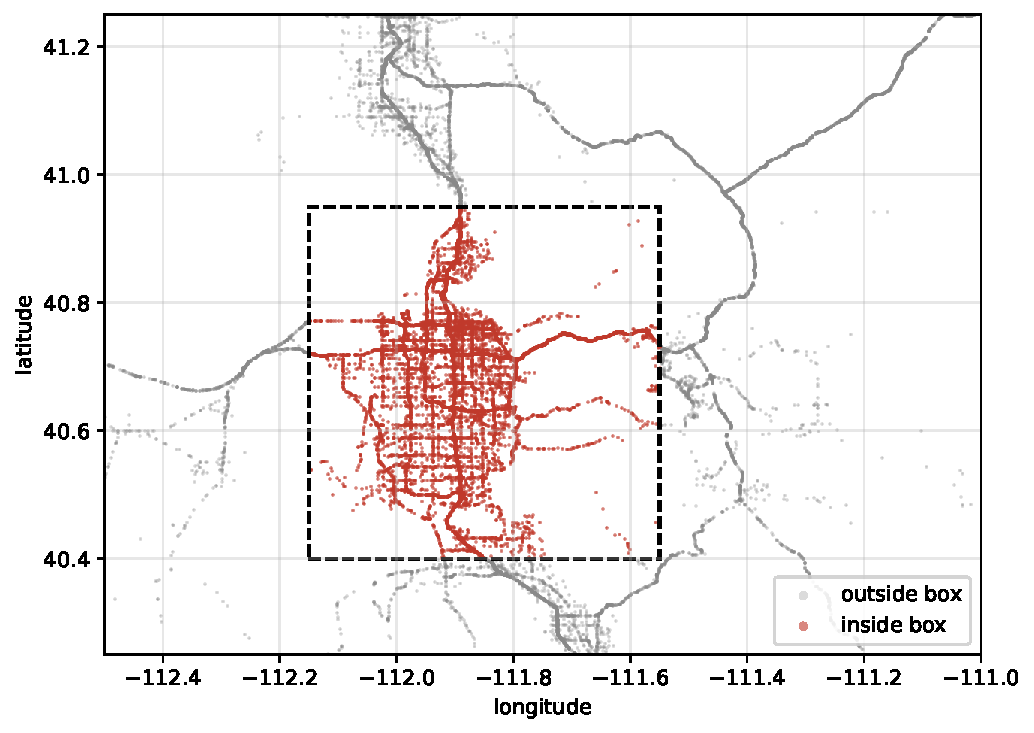
\includegraphics[width=0.75\linewidth]{figures/slc_extent.pdf}
\Description{Scatter of a random sample of raw GPS fixes
zoomed around the SLC bounding box; red fixes lie inside the
box, gray outside.}
\caption{Raw GPS fixes around the SLC bounding box (random
sample of $\sim\!10^{5}$ from $924$~M). Red points fall inside
the box ($40.4$--$40.95^{\circ}$N, $112.15$--$111.55^{\circ}$W,
dashed); gray fall outside.}
\label{fig:slc-extent}
\end{figure}

\subsection{Map-matching}
\label{sec:mapmatching}

We project the raw GPS fixes onto the road network with the
Leuven implementation~\cite{meert2018hmm,leuvenmapmatching} of
the hidden Markov map-matcher of Newson and
Krumm~\cite{newson2009hmm}. The matcher models the
GPS-to-link perpendicular distance as a zero-mean Gaussian with
standard deviation $\sigma$ (in metres); $\sigma$ is the only
emission parameter and is corpus-dependent. Newson and Krumm
fit $\sigma \approx 4.07$~m on their Seattle corpus; on our
sparser SLC corpus we refit by self-consistency. We re-run the
matcher across a range of candidate $\sigma$ (with a candidate
pruning radius \texttt{max\_dist} $= 400$~m, the matcher's
default upper bound on emission distance), compute the standard
deviation of the per-fix residuals over the surviving fixes,
and pick the smallest $\sigma$ at which the declared emission
std is no longer smaller than the measured one.

\begin{table}[H]
\centering
\caption{Self-consistency check for the GPS noise scale $\sigma$
on the SLC corpus.}
\label{tab:sigma-choice}
\scriptsize
\setlength{\tabcolsep}{6pt}
\begin{tabular}{cccl}
\toprule
$\sigma_{\textsf{declared}}$ & $\sigma_{\textsf{std}}$ (filtered)
   & gap $= \sigma_{\textsf{std}} - \sigma$ & verdict \\
\midrule
1.00 & 2.20 & $+1.20$ & too tight \\
1.75 & 2.77 & $+1.02$ & too tight \\
3.00 & 3.15 & $+0.15$ & slightly too tight \\
\textbf{3.50} & \textbf{3.22} & $\mathbf{-0.28}$
   & \textbf{first $\sigma > \sigma_{\textsf{std}}$ (chosen)} \\
3.75 & 3.25 & $-0.50$ & too loose \\
4.00 & 3.26 & $-0.74$ & too loose \\
5.00 & 3.31 & $-1.69$ & too loose \\
\bottomrule
\end{tabular}
\end{table}

\noindent The sign of $\sigma_{\textsf{std}} -
\sigma_{\textsf{declared}}$ flips between $\sigma = 3.0$ and
$\sigma = 3.5$. We therefore set $\sigma = 3.5$~m throughout
this paper.

\paragraph{Two map versions.}
The pipeline operates on two views of the same SLC road
network. The \emph{low-resolution} map is the MATSim simulator
network ($N \approx 99{,}716$ directed links). The
\emph{high-resolution} map is the same OSM extract with long or
curved MATSim links subdivided into shorter sub-edges so that
arterial geometry is captured by collinear sub-edges. The main
pipeline uses high-resolution matching aggregated to
low-resolution links; the low-res baseline of
\cref{sec:baselines} uses low-resolution matching instead.

\section{Popularity matrix}
\label{sec:counting}

The final stage of the pipeline aggregates the matched edge visits
into a sparse matrix $C \in \mathbb{Z}_{\ge 0}^{T \times N}$ that is the input
to the rest of the project. Each row corresponds to a time bin, each
column to a road link, and each entry counts the number of edge
visits that fell into that bin and link.

\subsection{Time bins}

Time is partitioned into non-overlapping bins of equal width
$\Delta = 300$~seconds (five minutes). For an absolute timestamp
$t$ measured in seconds since the epoch $t_0 = $~2018-01-01, the
bin index is
\begin{equation}
b(t) \;=\; \Big\lfloor \frac{t - t_0}{\Delta} \Big\rfloor.
\end{equation}
The binning is global: every matched fix produced anywhere in the
$30$-day observation window is mapped to the same time grid, which
contains $T = 30 \times 24 \times 12 = 8{,}640$ five-minute
bins.
A five-minute resolution is chosen to balance two competing
constraints: too coarse a bin (e.g.\ one hour) blurs the rush-hour
profile of the network; too fine a bin (e.g.\ one minute) leaves
the matrix excessively sparse, with most cells empty even on busy
links.

\subsection{Counting rule}
\label{sec:counting-rule}

The matched-fix output of \cref{sec:mapmatching} provides, for
each trip $r$, a list of pairs $(\textsf{lid}_j, t_j)$, one per
emitting GPS fix. The counting rule is:

\begin{enumerate}[leftmargin=2.0em]
  \item \textbf{Bin assignment.} Each pair is assigned to the bin
        \begin{equation}
          b_j \;=\; b\!\big(t_j\big)
              \;=\; \Big\lfloor \frac{t_j - t_0}{\Delta} \Big\rfloor.
        \end{equation}
  \item \textbf{Per-trip deduplication.} For a given trip $r$, all
        fixes that fall in the same bin and on the same link are
        collapsed into a single contribution. Concretely, the set
        of contributions from trip $r$ is the set of distinct
        triples
        \begin{equation}
          \big\{\,(b_j,\, \textsf{lid}_j,\, r) \;:\; j = 1, \ldots, M_r \,\big\}.
        \end{equation}
        If the same trip emits five fixes that all map to the same
        bin and the same link, that combination is counted exactly
        once.
  \item \textbf{Accumulation.} The popularity-matrix entry $C_{b, i}$
        is then the number of distinct trips that contributed at
        least one fix to bin $b$ on link $i$:
        \begin{equation}
        \label{eq:count-rule}
          C_{b, i} \;=\; \big|\,\{\, r \;:\;
                    \exists\, j \text{ with } b_j = b,\;
                                       \textsf{lid}_j = i \,\}\,\big|.
        \end{equation}
\end{enumerate}

The per-trip deduplication ensures that $C_{b, i}$ measures link
occupancy by distinct vehicles in the corpus, not the GPS-emission
density of those vehicles: a trip that produces several fixes while
crossing one link inside a single $5$-minute window contributes one
unit, not several.

\subsection{Sparse matrix representation}

The matrix $C$ has dimensions $T \times N \approx 8.6 \times 10^8$
cells, where $T = 8{,}640$ is the number of five-minute bins
(\cref{sec:counting}) and $N = 99{,}716$ is the number
of directed road links. Only a small fraction of these cells are
nonzero: at five-minute resolution most road links carry no trip
in any specific window. We therefore store $C$ in
compressed sparse row format alongside the per-row timestamps and
per-column link identifiers, which on the SLC corpus reduces the
artifact to roughly $7$~MiB.

\subsection{\texorpdfstring{What $C$ does and does not measure}{What C does and does not measure}}

The matrix $C$ summarizes how many trips, drawn from the
$714{,}594$-trip corpus, traversed each road link in each
five-minute window of the $30$-day observation period. It is a
direct empirical proxy for link usage and feeds the prior $E_b$
used in the two-phase {PageRank} chain.

Two limitations are worth stating up front. First, the corpus is a
biased sample of real traffic: it is drawn from a specific population
of GPS-emitting devices and is not a uniform sample of all vehicles
on the road. Links that systematically attract devices in the
sample (e.g.\ commercial freeway corridors) are over-represented
relative to links that attract a different population
(e.g.\ residential cul-de-sacs). The matrix should therefore be
read as a \emph{prior} on link usage, not as ground-truth volume.
Second, even within the corpus, sparsity is structural: at any
single five-minute slot, the median number of GPS fixes per link is
zero, and only a few hundred to a few thousand links carry any
matched visit at all. To quantify this at the bin-of-week level,
we aggregate the first four full weeks of the corpus ($8{,}064$
bins, i.e.\ $4 \times 7 \times 288$ five-minute slots) and ask, for
each \emph{(link, bin-of-week)} cell, in how many of the four
weeks it received at least one matched fix. The result is in
\cref{tab:justif-zeros}.

\begin{table}[H]
\centering
\caption{How often each (link, bin-of-week) cell was zero across
the four weeks. The cell is structurally empty if all four weeks
were zero. ``Active'' cells are the union of $k = 0, 1, 2, 3$
rows ($5.95 \times 10^{6}$ in total, about $3\%$ of all cells).
The total cell count $201{,}027{,}456 = N \times 2{,}016$
counts \emph{(link, bin-of-week)} pairs for a single week
($2{,}016 = 7 \times 288$ five-minute slots in a week); each
cell carries four observations, one per calendar week.}
\label{tab:justif-zeros}
\small
\begin{tabular}{lrr}
\toprule
weeks with zero count & cell count & fraction \\
\midrule
$k = 0$ (active in every week)            & $304{,}983$    & $0.15\%$ \\
$k = 1$                                    & $499{,}625$    & $0.25\%$ \\
$k = 2$                                    & $1{,}153{,}583$ & $0.57\%$ \\
$k = 3$                                    & $3{,}994{,}889$ & $1.99\%$ \\
$k = 4$ (never observed in $4$ weeks)     & $195{,}074{,}376$ & $97.04\%$ \\
\midrule
total                                      & $201{,}027{,}456$ & $100\%$ \\
\bottomrule
\end{tabular}
\end{table}

$97\%$ of all (link, bin-of-week) cells are zero in every one of
the four weeks; only $0.15\%$ are active in all four. Most of
the matrix is therefore not just sparse but \emph{structurally
empty}, and most ``active'' cells are active in only one of the
four weeks, i.e.\ represent a single noisy sample rather than a
stable rate. The downstream graph-diffusion smoothing described
elsewhere in the project addresses this by spreading mass to
network neighbors of observed links.

\section{Building the teleportation prior}
\label{sec:prior}

\subsection{From counts to a prior by row-normalization}

The matrix $C$ is converted into a per-bin
teleportation prior by row-normalization. For every bin $b$ with
$\sum_i C_{b, i} > 0$, define
\begin{equation}
E_b(i) \;=\; \frac{C_{b, i}}{\sum_{j} C_{b, j}}.
\end{equation}
This makes $E_b$ a probability distribution over the $N$ links of
the network: the share of trip-presence mass during bin $b$ that
landed on link $i$. Bins with no observed trips are assigned the
uniform distribution $E_b(i) = \frac{1}{N}$, which acts as an
uninformative fallback.

The construction of $E_b$ is the entire purpose of the pipeline
described above: every step from raw GPS in \cref{sec:dataset} to
the sparse matrix in \cref{sec:counting} contributes a piece of the
journey from a device-level point cloud to a link-level distribution
$E_b$ that the smoothing of \cref{sec:diffusion} regularizes and the
model of \cref{sec:model} consumes.

\subsection{Diffusion smoothing of the popularity prior}
\label{sec:diffusion}

The teleportation prior $E_b$ summarizes what was actually observed
on the road network during bin $b$, but it has two structural
shortcomings for predictive use. First, $E_b$ is sparse: a typical
$5$-minute window puts non-zero mass on only a few thousand of the
$N$ links, leaving the rest of the network at exact zero. Second, the empirical signal is noisy at fine
resolution: the same heavy corridor can be touched by zero observed
trips in one bin and several trips in the very next, simply because
no GPS device happened to emit a fix on that link inside that
$5$-minute slot.

We measure the scale of this noise from the four-week structure
of the corpus. For each (link, bin-of-week) cell that the corpus
saw at least once, we compute the standard deviation of its
normalized count $E_b(i) = C_{b,i} / \sum_j C_{b,j}$ across the
four weeks; this captures how much the same link in the same
time-of-week jitters from week to week. We call this per-cell
quantity $\NF_{b, i}$.

\jeff{State the units explicitly: $E_b(i)$ is the probability that
a GPS fix falling in bin $b$ lands on link $i$. The figure axis and
the text should both say that.}

\hamid{Concretely, $E_b(i) = C_{b, i} / \sum_j C_{b, j}$ is the
fraction of all GPS fixes recorded in bin $b$ that fell on link
$i$, i.e.\ the probability that a single fix drawn uniformly from
that 5-minute window lands on link $i$. The cross-week deviation
$\NF_{b, i}$ is the spread of that probability across the four
weeks at the matched bin-of-week; both quantities are
dimensionless probability mass.}

The median over the $5.95 \times 10^{6}$ active cells of
\cref{tab:justif-zeros} is $\NFG = 2.65 \times
10^{-4}$, a single corpus-wide scalar used as a global yardstick.
Differences in $E_b$ smaller than $\NF$ are not distinguishable
from week-to-week sampling noise; the smoothing step below is
calibrated to this scale.

\begin{figure}[H]
\centering
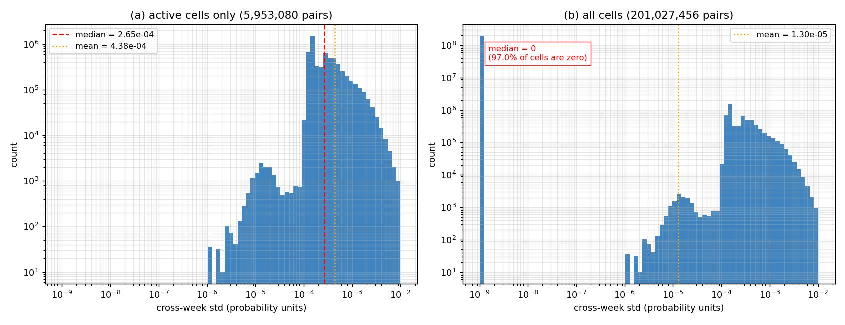
\includegraphics[width=0.85\linewidth,trim={0 0 203 0},clip]{figures/noise_floor_with_and_without_zeros.pdf}
\Description{Histogram of cross-week std values on the 5.95M active cells.}
\caption{Distribution of the cross-week standard deviation
$\NF_{b, i} = \mathrm{std}_w \, E_b^{(w)}(i)$ across the four
weeks, per (link, bin-of-week), restricted to the
$5.95 \times 10^{6}$ active cells. \hamid{Units on the horizontal
axis are dimensionless probability mass: a GPS-fix-on-link
probability $E_b(i) = C_{b,i} / \sum_j C_{b, j}$.}}
\label{fig:noise-floor-raw}
\end{figure}

{\color{blue}
\begin{figure}[H]
\centering
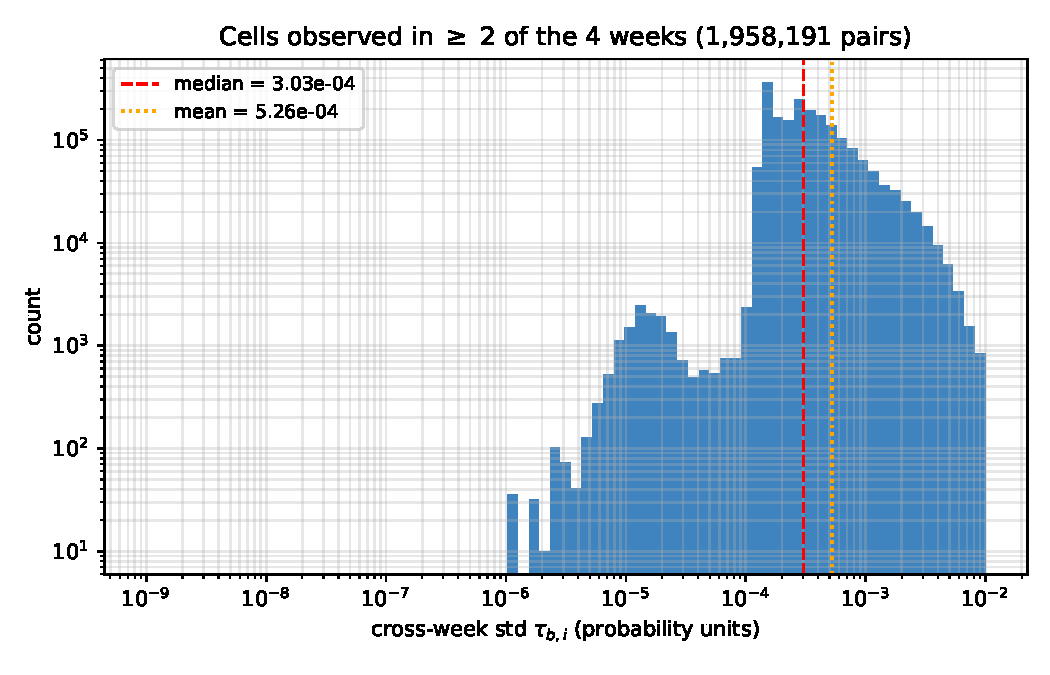
\includegraphics[width=0.75\linewidth]{figures/noise_floor_2plus_weeks.pdf}
\Description{Same histogram as the previous figure but restricted to cells observed in at least 2 of the 4 weeks. The spike at zero is gone.}
\caption{\textcolor{blue}{[temporary]} Same distribution as
\cref{fig:noise-floor-raw} but restricted to cells observed in
\emph{at least 2} of the 4 weeks ($1.96 \times 10^{6}$ pairs).
Removing the one-week-only cells (whose std collapses to a
near-zero spike) exposes the actual $\tau_{b,i}$ distribution.}
\label{fig:noise-floor-2plus}
\end{figure}
}

A graph-aware smoothing step addresses both issues at once. It
lifts every link to a positive value (so the prior never has hard
zeros) and borrows mass from neighboring links (so a heavy link
does not disappear because of an empty bin). The smoothing is
applied row by row to the count matrix
$C \in \mathbb{Z}_{\ge 0}^{T \times N}$ in three steps.

\paragraph{Laplace pseudo-count.}
\label{sec:laplace}

For every bin $b$ and every link $i$, replace the raw count by
\begin{equation}
\label{eq:laplace}
c_b(i) \;=\; C_{b, i} + \alpha,
\qquad \alpha = 10^{-2}.
\end{equation}
After this step every entry of $c_b$ is positive: the row is dense
before any further processing.

\paragraph{Single-step graph diffusion.}
\label{sec:diffusion-step}

Let $P \in \mathbb{R}^{N \times N}$ be the row-stochastic adjacency
matrix of the directed road graph: $P_{i, j} = \frac{1}{d^{\textsf{out}}_i}$
when there is a road link from $i$ to $j$, and zero otherwise; here
$d^{\textsf{out}}_i$ is the out-degree of link $i$. Apply one lazy
random-walk step on the graph,
\begin{equation}
\label{eq:diffuse}
\tilde c_b \;=\; (1 - \gamma)\, c_b \;+\; \gamma\, P\, c_b,
\qquad \gamma = 0.20,
\end{equation}
where $(P\, c_b)_i = \sum_{j} P_{i, j}\, c_b(j)$ is the average of
$c_b(j)$ over the out-neighbors $j$ of link $i$. The mass on link
$i$ is therefore averaged with the mass on the links it leads to.
Finally, normalize each row to a probability distribution:
\begin{equation}
\label{eq:diffused-prior}
\tilde E_b(i) \;=\; \frac{\tilde c_b(i)}{\sum_j \tilde c_b(j)}.
\end{equation}
The result $\tilde E_b \in \mathbb{R}^{N}$ is the
\emph{diffused prior}: dense, positive on every road link, and
preserving the order of the heaviest links across the corpus.
$\tilde E_b$ is used as an alternative to the raw $E_b$
throughout the evaluation of \cref{sec:evaluation}.

\paragraph{Choosing $\gamma$ from the noise floor.}
The diffusion strength $\gamma$ is not free. We pick it so that
the smoothing displaces any single cell by no more than half of
that cell's own week-to-week sampling noise: any larger move and
the smoother is overwriting structure with neighbor mass rather
than filling in noise. Concretely, for each
$(\text{link } i,\ \text{bin-of-week } b)$ cell with at least
one observed positive count across the four full corpus weeks
$w = 1, \ldots, W$, define the per-week displacement
\begin{equation}
\label{eq:displacement}
D^{(w)}_{b, i}(\gamma)
\;=\;
\Big| \, \tilde E^{(w)}_{b, i}(\gamma) - E^{(w)}_{b, i} \, \Big|,
\end{equation}
the cell-level displacement averaged across the four weeks
\begin{equation}
\label{eq:disp-avg}
D_{b, i}(\gamma)
\;=\;
\frac{1}{W} \sum_{w = 1}^{W} D^{(w)}_{b, i}(\gamma),
\end{equation}
and compare it to the cross-week noise floor
$\NF_{b, i}$ of the same cell. Both $D_{b, i}$ and $\NF_{b, i}$
are in probability units, so the ratio $D_{b, i} / \NF_{b, i}$
is \emph{dimensionless}: "displacement measured in units of one
noise-floor unit." The criterion is
\begin{equation}
\label{eq:gamma-criterion}
D_{b, i}(\gamma) \;\le\; \tfrac{1}{2}\, \NF_{b, i}.
\end{equation}
We compare each cell either against its own cross-week noise
scale $\NF_{b, i}$ (\emph{per-cell criterion}, one number per
active cell) or against the corpus-wide median noise scale
$\NFG = 2.65 \times 10^{-4}$
(\emph{global criterion}, a single scalar shared by every cell):
\begin{align}
\label{eq:gamma-criterion-pair}
\text{per-cell:}\quad
  & D_{b, i}(\gamma) \;\le\;
    \tfrac{1}{2}\, \NF_{b, i}, \\[2pt]
\text{global:}\quad
  & D_{b, i}(\gamma) \;\le\;
    \tfrac{1}{2}\, \NFG
    \;=\; 1.325 \times 10^{-4}.
\end{align}
On the active cells of the SLC corpus
($n_{\textsf{active}} = 5{,}954{,}929$, per-cell
$\NF$ median $= 2.3 \times 10^{-4}$),
\cref{tab:gamma-noise-floor} reports three quantiles of each
ratio: the median, the $95$th percentile, and the fraction of
cells whose ratio exceeds the half-noise threshold.

\begin{table}[H]
\centering
\caption{Quantiles of the dimensionless displacement-to-noise
ratio $D_{b, i}(\gamma) / \NF$ across the $5{,}954{,}929$
active SLC cells; left block uses the per-cell denominator
$\NF_{b, i}$, right block uses the global denominator
$\NFG = 2.65 \times 10^{-4}$. Read each row as
``at this $\gamma$, half / $95\%$ / fraction-above-$0.5$ of
active cells are displaced by at most so-many noise units.''
The criterion is the largest $\gamma$ whose $95$th-percentile
ratio stays $\le 0.5$.
\jeff{remove some of the columns}}
\label{tab:gamma-noise-floor}
\small
\setlength{\tabcolsep}{4pt}
\begin{tabular}{c|ccc|ccc}
\toprule
& \multicolumn{3}{c}{per-cell criterion}
& \multicolumn{3}{c}{global criterion} \\
\cmidrule(lr){2-4}\cmidrule(lr){5-7}
$\gamma$
 & med. & $95$th pct.\ & $>\!0.5$
 & med. & $95$th pct.\ & $>\!0.5$ \\
\midrule
$0.00$ & $0.000$ & $0.000$ & $0.00\%$ & $0.000$ & $0.000$ & $0.00\%$ \\
$0.05$ & $0.038$ & $0.100$ & $0.42\%$ & $0.034$ & $0.215$ & $0.90\%$ \\
$0.10$ & $0.069$ & $0.186$ & $1.00\%$ & $0.062$ & $0.393$ & $3.31\%$ \\
$0.12$ & $0.081$ & $0.219$ & $1.27\%$ & $0.073$ & $0.463$ & $4.40\%$ \\
$0.13$ & $0.087$ & $0.236$ & $1.41\%$ & $0.079$ & $0.498$ & $4.96\%$ \\
$0.14$ & $0.093$ & $0.253$ & $1.56\%$ & $0.084$ & $0.533$ & $5.53\%$ \\
$0.15$ & $0.099$ & $0.270$ & $1.73\%$ & $0.090$ & $0.568$ & $6.10\%$ \\
$\mathbf{0.20}$
       & $\mathbf{0.130}$ & $\mathbf{0.354}$ & $\mathbf{2.62\%}$
       & $\mathbf{0.117}$ & $\mathbf{0.741}$ & $\mathbf{8.95\%}$ \\
$0.25$ & $0.160$ & $0.436$ & $3.63\%$ & $0.144$ & $0.912$ & $11.87\%$ \\
$0.30$ & $0.190$ & $0.518$ & $5.39\%$ & $0.171$ & $1.081$ & $14.81\%$ \\
$0.40$ & $0.248$ & $0.680$ & $9.42\%$ & $0.224$ & $1.413$ & $20.64\%$ \\
$0.50$ & $0.306$ & $0.838$ & $17.29\%$ & $0.276$ & $1.737$ & $26.59\%$ \\
$0.70$ & $0.418$ & $1.145$ & $32.10\%$ & $0.376$ & $2.364$ & $37.83\%$ \\
\bottomrule
\end{tabular}
\end{table}

\begin{table}[H]
\centering
\caption{\textcolor{blue}{[temporary]} Displacement of zero cells
($n_{\textsf{zero}} = 1.95 \times 10^{8}$) in units of
$\NFG = 2.65 \times 10^{-4}$.}
\label{tab:gamma-zero-cells}
\small
\setlength{\tabcolsep}{6pt}
\begin{tabular}{cccc}
\toprule
$\gamma$ & median & $95$th pct.\ & $>\!0.5$ \\
\midrule
$0.00$ & $0.0004$ & $0.0004$ & $0.00\%$ \\
$0.05$ & $0.0004$ & $0.0004$ & $0.01\%$ \\
$0.10$ & $0.0004$ & $0.0004$ & $0.03\%$ \\
$0.12$ & $0.0004$ & $0.0004$ & $0.04\%$ \\
$0.13$ & $0.0004$ & $0.0004$ & $0.04\%$ \\
$0.14$ & $0.0004$ & $0.0004$ & $0.05\%$ \\
$0.15$ & $0.0004$ & $0.0004$ & $0.05\%$ \\
$\mathbf{0.20}$
       & $\mathbf{0.0004}$ & $\mathbf{0.0004}$ & $\mathbf{0.08\%}$ \\
$0.25$ & $0.0004$ & $0.0004$ & $0.10\%$ \\
$0.30$ & $0.0004$ & $0.0004$ & $0.13\%$ \\
$0.40$ & $0.0004$ & $0.0004$ & $0.20\%$ \\
$0.50$ & $0.0004$ & $0.0004$ & $0.28\%$ \\
$0.70$ & $0.0003$ & $0.0004$ & $0.46\%$ \\
\bottomrule
\end{tabular}
\end{table}

\noindent\textcolor{blue}{Reading the zero-cell table. The median
and $95$th-percentile ratios are essentially constant at
$\approx 4 \times 10^{-4}$ across all $\gamma$: at least $95\%$
of zero cells never see diffusion mass, they only carry the
Laplace floor $\alpha / N$. The fraction of zero cells exceeding
the half-noise tolerance is $0.08\%$ at $\gamma = 0.20$
($\sim 1.5 \times 10^{5}$ cells out of $1.95 \times 10^{8}$);
these are the cells immediately adjacent to active links and
they are the ones that get visibly filled in. The takeaway is
that the diffusion is bounded even on the cells where the
per-cell criterion of \cref{tab:gamma-noise-floor} is undefined:
it lifts a small adjacency-defined tail of zero cells into the
noise band and leaves the rest at the Laplace floor.}

\paragraph{Choice of $\gamma$.}
Under the per-cell criterion the $95$th-percentile ratio first
crosses $0.5$ between $\gamma = 0.25$ ($0.436$) and
$\gamma = 0.30$ ($0.518$), so
$\gamma_{\max}^{\textsf{pc}} \approx 0.25$. The stricter global
criterion crosses between $\gamma = 0.13$ ($0.498$) and
$\gamma = 0.14$ ($0.533$), giving
$\gamma_{\max}^{\textsf{global}} \approx 0.13$. We use
$\gamma = 0.20$ throughout the paper: it sits comfortably inside
the per-cell ceiling, the median active cell is displaced by
only $0.117 \, \NFG$ even under
the global criterion, and the $95$th-percentile ratio crosses
the half-noise bound only mildly ($0.741$).

\paragraph{Violator tail at $\gamma = 0.20$.}
To see how far past the tolerance the violators sit, we sweep
the threshold $\eta$ in
$D_{b, i}(0.20) > \eta \, \NFG$
across the active cells:

\begin{center}
\small
\begin{tabular}{ccccccc}
\toprule
$\eta$ & $0.2$ & $0.5$ & $0.8$ & $1.0$ & $1.5$ & $2.0$ \\
\midrule
fraction $>\eta\,\NFG$
       & $28.5\%$ & $8.9\%$ & $4.4\%$ & $3.0\%$ & $1.3\%$ & $0.6\%$ \\
\bottomrule
\end{tabular}
\end{center}

\noindent
The violator tail thins quickly: of the $8.9\%$ that exceed
half the noise floor, only $3\%$ exceed $\NFG$ and fewer than
$0.7\%$ exceed $2\,\NFG$, so the smoothing rarely changes a
cell by more than its own week-to-week jitter. The per-cell
and global criteria agree on the median and differ only on the
upper tail (the per-cell version self-normalizes against busy
cells, the global version measures every cell against the
corpus median); we report both and use $\gamma = 0.20$ as the
working compromise.


\section{Evaluation framework}
\label{sec:evaluation-framework}

We now fix the metrics and protocol used by every subsequent
evaluation, including the single-phase baseline of
\cref{sec:baseline-singlephase} and the two-phase chain of
\cref{sec:model}.

\subsection{Error measures}
\label{sec:error}

To evaluate a chain we compare two probability vectors over the
$N$ road links: a \emph{truth} vector $t$ and a \emph{prediction}
vector $p$, both summing to one (each entry is the share of
trip-presence mass on one link in a given bin). Two scalar
summaries are used.

\paragraph{Mean Relative Error (MRE).}
For a numerical regularizer $\varepsilon \ge 0$, define the
per-link relative error
\begin{equation}
\label{eq:mre-link}
r_i \;=\; \frac{|t_i - p_i|}{t_i + \varepsilon},
\end{equation}
which is dimensionless: numerator and denominator are both in
probability units, so $r_i$ measures error as a fraction of the
truth itself. We aggregate $r_i$ across every link in the
network:
\begin{equation}
\textsf{MRE}_{\textsf{overall}} \;=\; \frac{1}{N} \sum_{i = 1}^{N} r_i.
\end{equation}
The regularizer $\varepsilon$ is
needed only when $t$ has links with $t_i = 0$: it prevents division
by zero and acts as a numerical floor that controls how much
empty-truth links inflate the average. We report
$\varepsilon = 10^{-6}$ throughout, and additionally
$\varepsilon = 0$ in configurations where the diffused prior
$\tilde E_b$ guarantees $t_i > 0$ on every link.

\hamid{To anchor the scale, \cref{tab:fixes-per-bin} summarizes the
number of matched GPS fixes in each $5$-minute bin across the
$8{,}640$ bins of the corpus. The busiest bin contains
$M_{\max} = 20{,}881$ fixes, so the smallest possible nonzero
per-link probability anywhere in the corpus is
$1 / M_{\max} \approx 4.8 \times 10^{-5}$. With the uniform
per-link probability $1 / N \approx 1.00 \times 10^{-5}$ and the
empirical noise floor
$\NFG = 2.65 \times 10^{-4}$,
our $\varepsilon = 10^{-6}$ sits below all three: it stabilizes
the denominator for links with $t_i = 0$ without otherwise
perturbing the links we care about.}
\jeff{why $\varepsilon = 10^{-6}$}

\begin{table}[H]
\centering
\caption{Matched GPS fixes per $5$-minute bin across the
$8{,}640$ bins of the corpus.}
\label{tab:fixes-per-bin}
\small
\begin{tabular}{lr}
\toprule
statistic & value \\
\midrule
total matched fixes & $58{,}410{,}362$ \\
\midrule
min                 & $295$ \\
$10$th percentile   & $1{,}405$ \\
median              & $4{,}823$ \\
mean                & $6{,}760$ \\
$90$th percentile   & $14{,}746$ \\
max                 & $20{,}881$ \\
\bottomrule
\end{tabular}
\end{table}

\paragraph{Three comparisons.}
For every target bin $t$ in the evaluation sample we compute the
chain's prediction $\hat v(t)$ by running the iteration
\eqref{eq:iter} until convergence with $E_b(t)$ (or $\tilde E_b(t)$)
as the teleportation prior. We then form three (truth, prediction)
pairs:

\begin{enumerate}
  \item \textbf{dataset $\to$ dataset} (week to next week): truth
        $= E_b(t + 7~\text{days})$, prediction $= E_b(t)$. Reports
        the natural week-to-week variability of the empirical
        signal at the same weekday and hour-of-day; serves as the
        \emph{noise floor} the model needs to beat.
  \item \textbf{dataset $\to$ model} (forecast next week): truth
        $= E_b(t + 7~\text{days})$, prediction $= \hat v(t)$.
        Reports how well the chain, fed this week's prior,
        predicts next week's empirical signal.
\end{enumerate}
With the diffused prior, the same two comparisons replace
$E_b$ by $\tilde E_b$ on \emph{both sides}: the truth vector,
the prediction vector when the prediction is itself a prior
(comparison 1), and the chain input that produces $\hat v(t)$
(comparison 2) are all diffused before the MRE is taken. This
keeps every comparison apples-to-apples within a single choice
of prior.

\paragraph{Sampling protocol.}
For each of the seven days of the week (Mon, $\ldots$, Sun) we
draw $120$ source bins uniformly at random, for a total of
$7 \times 120 = 840$ target bins. A bin is eligible only if
both the bin itself and its $+7$-day sibling exist in the
matrix. In our $30$-day corpus this restricts source bins to
days $1$--$23$ (Sept~$1$ to Sept~$23$) paired with siblings in
days $8$--$30$ (Sept~$8$ to Sept~$30$); the source bins
therefore span weeks $1$--$3$ and the first days of week $4$,
not just the first week. The seed is fixed ($7$), so the
sample is identical across configurations.


\section{Baseline: single-phase PageRank}
\label{sec:baseline-singlephase}

The most natural baseline on the popularity prior $E_b$ is the
single-phase PageRank chain with $E_b$ as the
teleportation distribution. Given the row-stochastic adjacency
$P$ of the directed road graph (each row of $P$ being uniform over
the outgoing road neighbors of one link) and a teleport
probability $p \in (0, 1)$, the iteration is
\begin{equation}
\label{eq:single-phase-iter}
v_{n+1} \;=\; p\,E_b \;+\; (1 - p)\,P^{\top}\,v_n,
\end{equation}
applied until $\|v_{n+1} - v_n\|_1 < 10^{-7}$, with a safety cap
of $300$ iterations. The cap is conservative: the power
iteration converges geometrically at rate $1 - p$, so the
theoretical worst-case number of iterations to reach L1 error
$10^{-7}$ is
\begin{equation}
\label{eq:iter-bound}
n^{\star} \;=\; \frac{\ln 10^{-7}}{\ln (1 - p)}
\;=\; \frac{\ln 10^{-7}}{\ln 0.9492} \;\approx\; 310,
\end{equation}
which sits just above $300$. We checked empirically on $1{,}500+$
random target bins and the chain converged before $300$ iterations
in every single case; the observed maximum was $254$ iterations and
the median was $209$.
The cap is therefore never hit in practice and the recorded
results are at full $10^{-7}$ tolerance throughout. At every step
the walker teleports back to the prior with probability $p$ and
otherwise takes a uniform random step along an outgoing road
edge. The stationary distribution $v^{\star}$ of
\eqref{eq:single-phase-iter} is the single-phase prediction for
bin $b$.

\paragraph{Calibrating $p$ from the trip corpus.}
The chain in \eqref{eq:single-phase-iter} is a geometric absorption
process: the number of graph steps before a teleport is
$\textsf{Geom}(p)$ on $\{0, 1, 2, \ldots\}$ with mean
$\frac{1 - p}{p}$. We match $p$ to the empirical mean trip length
$\mathbb{E}[K_{\textsf{total}}]$ by method-of-moments, exactly as
the two-phase chain matches $\beta$ and $\rho$ to the per-phase
lengths:
\begin{equation}
\label{eq:single-phase-p}
p \;=\; \frac{1}{1 + \mathbb{E}[K_{\textsf{total}}]}.
\end{equation}
On the noise=3.5 matched corpus
($714{,}594$ trips, all route lengths), the empirical mean is
$\mathbb{E}[K_{\textsf{total}}] = 18.68$, which gives
$p = 0.0508$. The chain has only this one free parameter; the
``damping factor'' $1 - p = 0.9492$ that some authors report
is just a relabeling. \Cref{fig:single-phase-hist} shows the
empirical $K_{\textsf{total}}$ histogram with the
$\textsf{Geom}(p = 0.0508)$ reference overlaid.

\begin{figure}[H]
\centering
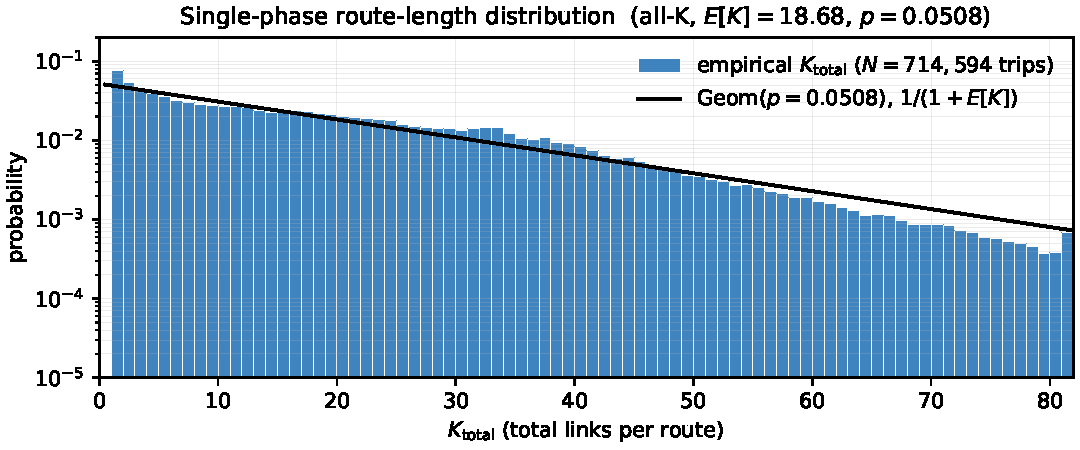
\includegraphics[width=\linewidth]{figures/single_phase_histogram.pdf}
\Description{Log-y histogram of the per-trip total link count
K_total on the noise=3.5 matched corpus of 714,594 trips, overlaid
with a geometric reference curve at p=0.0508.}
\caption{Empirical histogram of trip length $K_{\textsf{total}}$
on the $714{,}594$-trip corpus, with the matched
$\textsf{Geom}(p = 0.0508)$ overlay.}
\label{fig:single-phase-hist}
\end{figure}

\paragraph{Why this is a fair baseline.}
Three reasons. First, single-phase PageRank is the standard
graph-walk model on top of which the two-phase chain is built, so
the two share a graph, a prior $E_b$, and a power-iteration solver;
the only structural difference is the absence (single-phase) or
presence (two-phase) of an up$\to$down split. Second, the teleport
parameter $p$ is calibrated from the same trip corpus by the same
method-of-moments estimator that yields $\beta$ and $\rho$, so the
comparison is not penalized by an artificially detuned baseline.
Third, the baseline runs on the same $840$ target bins, the same
metric, and the same three comparisons as the two-phase chain, per
the evaluation contract.

\subsection{Why single-phase fails on our data}
\label{sec:whyfails-singlephase}

Evaluating \eqref{eq:single-phase-iter} on the same $840$ target
bins as \cref{tab:eval} ($120$ per weekday, seed $7$, all three
eps configurations) gives the numbers in
\cref{tab:single-phase}.

\begin{table}[H]
\centering
\caption{Single-phase PageRank baseline (chain
\eqref{eq:single-phase-iter} with $p = 0.0508$) on
$840$ target bins ($120$ per weekday, seed $7$). Conventions
match \cref{tab:eval}.}
\label{tab:single-phase}
\setlength{\tabcolsep}{6pt}
\renewcommand{\arraystretch}{1.30}
\begin{tabular}{@{}lccc@{}}
\toprule
Comparison
& \shortstack[c]{No diffusion\\$\varepsilon\!=\!10^{-6}$}
& \shortstack[c]{Diffused\\$\varepsilon\!=\!10^{-6}$}
& \shortstack[c]{Diffused\\$\varepsilon\!=\!0$} \\
\midrule
1. dataset$\to$dataset (next week) & $5.82$ & $0.68$ & $0.90$ \\
2. dataset$\to$model (forecast)    & $8.70$ & $1.07$ & $1.46$ \\
\bottomrule
\end{tabular}
\end{table}

Two readings of \cref{tab:single-phase}, paired against the
two-phase numbers in \cref{tab:eval}.

\paragraph{The forecast loses to the noise floor.}
Forecast Overall MRE is $1.07$ against a noise floor of $0.68$
(diffused, $\varepsilon = 10^{-6}$). The single-phase chain
therefore fails the contract's pass criterion that forecast
must not be worse than last-week-at-the-same-slot. The
two-phase chain in \cref{tab:eval} reaches forecast Overall MRE
of $1.04$ on the same comparison, only marginally better than
the single-phase baseline.

\paragraph{Why the single-phase mixes too much.}
At $p = 0.0508$ the chain takes on average
$\frac{1}{p} = 19.7$ graph steps before teleporting back to
$E_b$, which is the empirical mean trip length, so the chain is
calibrated to the right time scale. But $19.7$ uniform random
steps on the SLC road graph are enough to delocalize the
walker's distribution across the network: the steady state of a
random walk on a connected graph is the degree-proportional
distribution, and even at finite damping the chain has visibly
relaxed away from $E_b$ on the heavy links. The two-phase split
absorbs that mixing into the down phase ($\rho = 0.101$ leak)
while keeping the up phase close to $E_b$ ($\beta = 0.102$ leak,
applied on $P^{\uparrow}$ rather than the uniform $P$), which is
why the two-phase chain in \cref{tab:eval} preserves the
heavy-traffic head where the single-phase baseline does not. The next section formalizes this two-phase chain.

\section{Two-phase {PageRank} chain}
\label{sec:model}

The two-phase chain of this section turns a popularity prior (the
raw $E_b$ from \cref{sec:counting} or the diffused $\tilde E_b$
from \cref{sec:diffusion}) into a per-link prediction by running a
discrete-time Markov chain on a road-network state space. Its
design departs from a single-phase chain (one state per link) in
one important respect: each road link $i \in \{1, \ldots, N\}$ is
represented by \emph{two} states, an \emph{up-phase} state
$i^{\uparrow}$ and a \emph{down-phase} state $i^{\downarrow}$, so
the chain has $2N$ states in total. The doubled state space lets
the chain track two distinct regimes that a vehicle on the network
can occupy, and lets each regime contribute its own characteristic
mass to the link-level prediction.

\subsection{What the two phases represent}
\label{sec:two-phases}

The two phases of the chain correspond to two qualitatively
different regimes of a vehicle's behavior on the road network:

\begin{itemize}
  \item The \emph{up phase} represents a vehicle that has just
        appeared in the network and is choosing where to go: it has
        not yet committed to traveling along a specific corridor.
        Steps within the up phase let mass redistribute along the
        graph before any actual travel begins.
  \item The \emph{down phase} represents a vehicle that is
        \emph{traveling} along the network, advancing from one link
        to the next according to road geometry. Steps within the
        down phase trace out the kind of multi-link path that a real
        trip would follow.
\end{itemize}

A single-phase Markov chain on the $N$ physical links cannot
distinguish these two regimes: it would force a single transition
rule to govern both ``where does mass come from'' and ``where does
mass travel to'', and any stationary distribution it produced would
fold the two contributions into one number per link. The two-phase
chain keeps them separate, so that the steady-state mass on each
physical link decomposes into a contribution from up-phase
deliberation and a contribution from down-phase travel, both
controlled by their own transition rule. The next subsections
specify those transition rules and the parameters that govern them.

\subsection{Transition rule}
\label{sec:transition}

The state space is $\{1, \ldots, N\} \times \{\uparrow, \downarrow\}$:
every road link $i$ is duplicated into an up-state $i^{\uparrow}$
and a down-state $i^{\downarrow}$. A mass vector on this space is
a probability over $2N$ entries (it sums to one), and the chain's
stationary distribution decomposes naturally into an up-phase
share $v^{\uparrow}(i)$ and a down-phase share $v^{\downarrow}(i)$
per link.

The chain is fully specified by the rule that takes a current state
to its next state. From an up-phase state $i^{\uparrow}$ the rule is
\begin{itemize}
  \item with probability $1 - \beta$, the chain stays in the up
        phase and moves to one of $i$'s graph neighbors
        $j^{\uparrow}$, with the choice governed by an up-phase
        transition matrix $P^{\uparrow} \in \mathbb{R}^{N \times N}$;
  \item with probability $\beta \in (0, 1)$, the chain commits to
        traveling along link $i$ and moves to the down-phase state
        $i^{\downarrow}$ on the same link.
\end{itemize}
From a down-phase state $i^{\downarrow}$ the rule is
\begin{itemize}
  \item with probability $1 - \rho$, the chain stays in the down
        phase and moves to a graph neighbor $j^{\downarrow}$,
        governed by a down-phase transition matrix
        $P^{\downarrow} \in \mathbb{R}^{N \times N}$;
  \item with probability $\rho \in (0, 1)$, the trip ends and the
        chain teleports back to a fresh up-phase state drawn from
        the prior $E_b$: it jumps to $j^{\uparrow}$ with probability
        $E_b(j)$.
\end{itemize}
We adopt the \emph{column-stochastic} convention throughout: column
$i$ of any of these matrices stores the probability distribution
over next states, given that the chain is currently in state $i$.
In particular, $P^{\uparrow}$ and $P^{\downarrow}$ are column-stochastic
matrices supported on the directed road graph: the entry
$P^{\uparrow}_{j, i}$ is the probability of moving to link $j$ from
link $i$ in the up phase, and is zero whenever there is no road
link from $i$ to $j$ (and similarly for $P^{\downarrow}$). Below,
$v$ denotes the chain's mass vector at iteration step $n$; like
$E_b$, it is a probability over the $2N$ states (so
$\sum_i v^{\uparrow}(i) + \sum_i v^{\downarrow}(i) = 1$). The
chain's prediction for link $i$ is the sum
$v^{\uparrow}(i) + v^{\downarrow}(i)$, itself a probability over
the $N$ links.

The explicit construction of $P^{\uparrow}, P^{\downarrow}$ is as
follows. Each link $\ell$ in the
network carries two physical attributes from the graph: a free
flow speed $s(\ell)$ and a lane count $\lambda(\ell)$. Let
$\bar s(\ell) = s(\ell)/\bar s$ and
$\bar \lambda(\ell) = \lambda(\ell)/\bar \lambda$ denote these
attributes normalized by their per-link mean over the network,
and define the per-link physics weight
\begin{equation}
\label{eq:phase-weight}
w^{\uparrow}(\ell)
\;=\; \bar s(\ell)^{\alpha_s}\,\bar \lambda(\ell)^{\alpha_l},
\qquad
w^{\downarrow}(\ell)
\;=\; \bar s(\ell)^{-\alpha_s}\,\bar \lambda(\ell)^{-\alpha_l},
\end{equation}
with two real exponents $\alpha_s, \alpha_l \in \mathbb{R}$ that
parametrize how strongly the chain favors fast or wide links in
each phase. Each kernel is then a $w$-weighted row-stochastic
walk on the directed road graph, made column-stochastic by
transpose:
\begin{equation}
\label{eq:phase-kernel}
P^{\uparrow}_{j, i}
\;=\;
\frac{w^{\uparrow}(j)\,\mathbf{1}\!\left[\, i \to j \,\right]}
     {\sum_{j' : i \to j'} w^{\uparrow}(j')},
\end{equation}
where $i \to j$ denotes ``there is a directed road link from $i$
to $j$''; $P^{\downarrow}_{j, i}$ is defined identically with
$w^{\downarrow}$ in place of $w^{\uparrow}$. The down-phase
weight is the up-phase weight with $(\alpha_s, \alpha_l)$
sign-flipped, so the two phases are mirrored: when the up phase
prefers slow or narrow links the down phase prefers fast or wide
links, and vice versa. The default chain used throughout the
evaluation has $\alpha_s = \alpha_l = 0$, which makes
$w^{\uparrow}, w^{\downarrow} \equiv 1$ and both kernels reduce
to the uniform-over-out-neighbors walk on the directed road
graph; the speed/lane exponents come back as tuning knobs in the
intervention experiment of \cref{sec:intervention}.

Equivalently, ordering the $2N$ states as
$\big(1^{\uparrow}, \ldots, N^{\uparrow},\,
      1^{\downarrow}, \ldots, N^{\downarrow}\big)$,
the transition matrix of the chain is the column-stochastic
$2N \times 2N$ block matrix
\begin{equation}
\label{eq:M-block}
M_b \;=\;
\begin{pmatrix}
(1 - \beta)\, P^{\uparrow} & \rho\, E_b\, \mathbf{1}^{\top} \\[6pt]
\beta\, I                  & (1 - \rho)\, P^{\downarrow}
\end{pmatrix},
\end{equation}
where $I$ is the $N \times N$ identity, $\mathbf{1} \in
\mathbb{R}^{N}$ is the all-ones column vector, and $E_b \in
\mathbb{R}^{N}$ is the teleportation prior treated as a column
vector. The rank-1 block $\rho\, E_b\, \mathbf{1}^{\top}$ encodes
the ``every down-state gives mass back to the up phase via the same
prior $E_b$'' rule: each of its columns is the column vector
$\rho\, E_b$. With this convention the chain's mass distribution
$v \in \mathbb{R}^{2N}$ evolves as the simple matrix-vector product
\begin{equation}
\label{eq:iter}
v_{n+1} \;=\; M_b\, v_n,
\end{equation}
with no transpose required at any step of the iteration.

The two scalars $\beta$ and $\rho$ control how long the chain
stays in each phase before switching. A small $\beta$ lets the
up-phase walk redistribute mass over many graph neighbors before
committing to travel, while a small $\rho$ lets a single down-phase
trip extend over many links before restarting. The values used in
practice are not free parameters: they are method-of-moments
estimates from the trip corpus,
$\beta = \frac{1}{1 + \mathbb{E}[L_{\uparrow}]}$ and
$\rho = \frac{1}{1 + \mathbb{E}[L_{\downarrow}]}$, where
$L_{\uparrow}$ and $L_{\downarrow}$ are the empirical up- and
down-phase clock lengths of the matched corpus. Their derivation
from the raw matched routes is the subject of
\cref{sec:beta-rho-calibration}.

\subsection{Calibrating $\beta$ and $\rho$ from the trip corpus}
\label{sec:beta-rho-calibration}

The two scalars are not tuned against the evaluation metric; they
are read off the empirical distribution of trip lengths in the
matched-route corpus, in three steps.

\paragraph{Per-trip peak split.}
Every matched route is a sequence of road links
$(\ell_1, \ell_2, \ldots, \ell_K)$ produced by the Viterbi pass of
\cref{sec:mapmatching}. For each trip we identify a single \emph{peak link}
$\ell_{p}$ as the link with the largest score $s(\ell) =
\texttt{freespeed}(\ell) \times \texttt{numLanes}(\ell)$, with ties
broken by the link closest to the trip's middle. The peak link
plays the role of the trip's fastest, highest-capacity segment, the
freeway core of a typical commute. The two phases of the chain are
then defined as the prefix and the suffix of the route relative to
this peak,
\begin{equation}
\label{eq:phase-split}
L_{\uparrow} \;=\; \big|\{\,j \,:\, j < p\,\}\big|,
\qquad
L_{\downarrow} \;=\; \big|\{\,j \,:\, j > p\,\}\big|,
\end{equation}
so that $L_{\uparrow}$ counts the links traversed before the peak
(exclusive), $L_{\downarrow}$ counts the links traversed after the
peak (exclusive), and the peak link itself contributes the single
intermediate transition $i^{\uparrow} \to i^{\downarrow}$ of
\cref{sec:transition}; in particular,
$L_{\uparrow} + 1 + L_{\downarrow} = K$. By construction
$L_{\uparrow}, L_{\downarrow} \in \{0, 1, 2, \ldots\}$: a route
can begin or end on its own peak link, in which case the
corresponding phase has length zero. Short trips ($K = 1, 2$) are
handled by the convention $p = 0$ (the trip's first link is its own
peak), which yields $L_{\uparrow} = 0$ and $L_{\downarrow} = K - 1$
and contributes naturally to the empirical distributions. All
$714{,}594$ matched routes are therefore included in the
calibration sample.

\paragraph{Empirical distribution and method-of-moments.}
\Cref{fig:phase-histograms} shows the histograms of $L_{\uparrow}$
and $L_{\downarrow}$ on this sample, with a geometric reference
curve overlaid in black on each panel. Both empirical
distributions are heavy at zero and decay roughly exponentially,
which is the signature of a geometric distribution on
$\{0, 1, 2, \ldots\}$ with success probability $p$ and mean
$\frac{1 - p}{p}$. The black curves overlay $\textsf{Geom}(p)$
with $p$ matched to the empirical mean through
\begin{equation}
\label{eq:mom}
\mathbb{E}[L] \;=\; \frac{1 - p}{p}
\;\Longleftrightarrow\;
p \;=\; \frac{1}{1 + \mathbb{E}[L]},
\end{equation}
which is the method-of-moments estimator for a geometric on
$\{0, 1, \ldots\}$. Read each histogram bin as ``in this many
trips the prefix (resp.\ suffix) was exactly $L$ links long.''
Setting $\beta = 1 / (1 + \mathbb{E}[L_\uparrow])$ means the
chain's average up-phase clock length matches the empirical mean,
and likewise for $\rho$; the values $\beta, \rho \approx 0.10$
correspond to chains that stay in each phase about ten steps on
average. Reading the empirical means off the histograms,
\begin{equation}
\label{eq:phase-means}
\mathbb{E}[L_{\uparrow}] \;=\; 8.81,
\qquad
\mathbb{E}[L_{\downarrow}] \;=\; 8.87,
\end{equation}
and applying \eqref{eq:mom} to each phase yields
\begin{equation}
\label{eq:beta-rho}
\beta \;=\; \frac{1}{1 + \mathbb{E}[L_{\uparrow}]} \;=\; 0.102,
\qquad
\rho \;=\; \frac{1}{1 + \mathbb{E}[L_{\downarrow}]} \;=\; 0.101.
\end{equation}
These are the values fed into the chain in
\cref{sec:transition,sec:evaluation}; they are not chosen to fit
the evaluation, only to match the average up- and down-phase clock
lengths of the matched corpus. Both panels of
\cref{fig:phase-histograms} are well described by their geometric
reference in the body across the full range, with the empirical
bars sitting close to the geometric line throughout (a small
under-dispersion at large $L$ shows up as the bars being slightly
below the reference for $L_{\uparrow}, L_{\downarrow} \gtrsim 30$).

\begin{figure}[H]
\centering
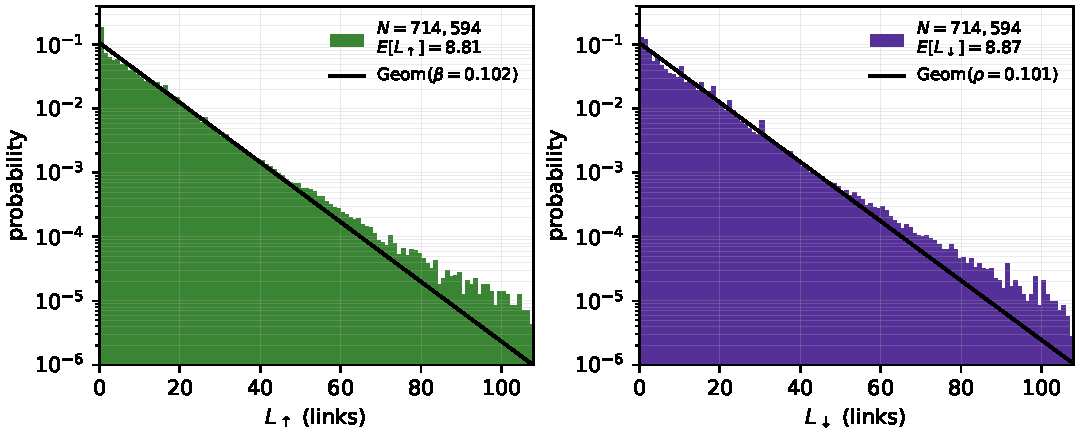
\includegraphics[width=\linewidth]{figures/phase_histograms_all_K.pdf}
\Description{Two side-by-side log-y histograms of the empirical
up-phase length L_up (left, green) and down-phase length L_down
(right, purple), each overlaid with a geometric reference curve
matched to the empirical mean.}
\caption{Empirical histograms of $L_{\uparrow}$ (left) and
$L_{\downarrow}$ (right) on the full $714{,}594$-trip matched
corpus, with the matched geometric overlay in black.}
\label{fig:phase-histograms}
\end{figure}

\paragraph{Why the geometric is the right reference.}
In the chain of \cref{sec:transition}, the number of up-phase
steps before the chain commits to travel is, by construction, a
geometric random variable with success probability $\beta$ on the
support $\{0, 1, 2, \ldots\}$, and the number of down-phase steps
before the chain restarts is geometric with probability $\rho$ on
the same support. Calibrating $\beta$ and $\rho$ by the
method-of-moments \eqref{eq:mom} therefore guarantees that the
chain matches the empirical mean phase length exactly. The
geometric assumption is approximate (the empirical tails are
slightly heavier than geometric, as visible in
\cref{fig:phase-histograms}), but the two means are by
construction correct, which is the moment that the chain
consumes.

\paragraph{Quantifying the fit.}
We pair the visual fit of \cref{fig:phase-histograms} with the
Kolmogorov-Smirnov statistic
$D = \sup_{k} \left| F_{\textsf{emp}}(k) - F_{\textsf{geom}}(k; p) \right|$,
where
\[
  F_{\textsf{emp}}(k)
  = \frac{1}{n} \sum_{i=1}^{n} \mathbf{1}\!\left[\, X_i \leq k \,\right]
\]
is the empirical CDF over the $n$ observed phase lengths
$\{X_i\}_{i=1}^{n}$,
\[
  F_{\textsf{geom}}(k; p) = 1 - (1 - p)^{k+1}, \qquad k \in \{0, 1, 2, \ldots\},
\]
is the CDF of the fitted geometric, and
\[
  p = \frac{1}{1 + \mathbb{E}[L]}
\]
is its maximum-likelihood estimator. Smaller $D$ means a tighter empirical
match. \Cref{tab:geom-fit} reports $D$ in three configurations.
Column $D_{\textsf{single}}$ fits one geometric to the full
route length $K = L_{\uparrow} + 1 + L_{\downarrow}$; columns
$D_{\uparrow}$ and $D_{\downarrow}$ fit geometrics to
$L_{\uparrow}$ and $L_{\downarrow}$ separately. The first row
matches on the low-resolution map and aggregates to
low-resolution links; the second matches on the
high-resolution map and aggregates to the same links; the
third both matches and aggregates at high-resolution.

\begin{table}[H]
\centering
\caption{Kolmogorov-Smirnov distance $D$ between empirical
phase lengths and the fitted geometric. Lower is better;
read each row as ``fitting a $\textsf{Geom}(p)$ to the
$L_\uparrow$ (resp.\ $L_\downarrow$) histogram leaves a $D$ of
this size under K-S.''}
\label{tab:geom-fit}
{\scriptsize
\setlength{\tabcolsep}{4pt}
\renewcommand{\arraystretch}{1.20}
\begin{tabular}{@{}llrccc@{}}
\toprule
Matcher & Granularity & $n$
  & $D_{\textsf{single}}$
  & $D_{\uparrow}$
  & $D_{\downarrow}$ \\
\midrule
low-res  & low-res links      & $293{,}066$ & $0.188$ & $0.129$ & $0.103$ \\
high-res & low-res links      & $621{,}986$ & $0.129$ & $\mathbf{0.030}$ & $\mathbf{0.032}$ \\
high-res & high-res sub-edges & $306{,}659$ & $0.102$ & $0.138$ & $0.148$ \\
\bottomrule
\end{tabular}
}
\end{table}

Two findings follow. On the low-resolution aggregation that
the chain runs on, splitting the route at the
$\textsf{freespeed} \times \textsf{permlanes}$ peak reduces $D$
by $76\%$ relative to the single-geometric fit, and the
matching change from the low-resolution to the high-resolution
map tightens $D_{\uparrow}$ and $D_{\downarrow}$ by a further
$76\%$ and $69\%$ on the same granularity. The empirical
variance moves the same way: the overdispersion ratio
$\frac{\operatorname{Var}(L_{\uparrow})}{\mathbb{E}[L_{\uparrow}](1 + \mathbb{E}[L_{\uparrow}])}$
moves from $2.07$ on the low-resolution map to $0.93$ on the
high-resolution map, sitting just below unity (slight
under-dispersion) and well inside the geometric model's natural
variance range.

At high-resolution sub-edge granularity, neither single nor
split geometric is a good fit; the empirical variance is
overdispersed by a factor of $1.8$ to $2.0$ and the up versus
down split, computed at low-resolution before being projected
to sub-edges, does not separate the empirical distribution
cleanly. We therefore keep the geometric calibration at
low-resolution ($\beta = 0.102$, $\rho = 0.101$) and treat the
high-resolution view of the same data as a descriptive
aggregation only.

\section{Experiments}
\label{sec:experiments}

The evaluation framework
(\cref{sec:evaluation-framework}) defines the metric (Overall
MRE), the two comparisons (dataset-to-dataset, forecast), and
the $840$-bin sampling protocol used by every table below.

\subsection{Evaluation results}
\label{sec:evaluation}

\Cref{tab:eval} reports the three comparisons in three
configurations: raw prior with $\varepsilon = 10^{-6}$, diffused
prior with $\varepsilon = 10^{-6}$, and diffused prior with
$\varepsilon = 0$. The chain uses the calibrated parameters
$\beta = 0.102, \rho = 0.101$ and $P^{\uparrow}, P^{\downarrow}$
uniform over outgoing road-graph neighbors. Iteration tolerance
is $10^{-7}$, maximum $300$ iterations.

\begin{table}[H]
\centering
\caption{Overall MRE of the two-phase chain across $840$
random target bins ($120$ per day of the week) on the SLC corpus.
$\beta=0.102, \rho=0.101$. Lower is better. ``No diffusion''
uses the raw prior $E_b$ of \cref{sec:counting}; ``Diffused''
uses the diffused prior $\tilde E_b$ of \cref{sec:diffusion}.}
\label{tab:eval}
\setlength{\tabcolsep}{6pt}
\renewcommand{\arraystretch}{1.30}
\begin{tabular}{@{}lccc@{}}
\toprule
Comparison
& \shortstack[c]{No diffusion\\$\varepsilon\!=\!10^{-6}$}
& \shortstack[c]{Diffused\\$\varepsilon\!=\!10^{-6}$}
& \shortstack[c]{Diffused\\$\varepsilon\!=\!0$} \\
\midrule
1. dataset$\to$dataset (next week) & $5.82$ & $\mathbf{0.68}$ & $0.90$ \\
2. dataset$\to$model (forecast)    & $8.53$ & $1.04$ & $1.42$ \\
\bottomrule
\end{tabular}
\end{table}

Two readings of the table.

\paragraph{Forecast sits above the noise floor.}
Row $2$ forecast Overall MRE is $1.04$, above the noise floor of
row $1$ at $0.68$. The chain's forecast of next week's signal is
therefore worse than last-week-at-the-same-slot. Since the chain
has no temporal dynamics (no time index in $M_b$ except through
the prior of the target bin), improving forecast performance
would require additional signal: weekly periodicity, multi-bin
context, or external covariates, none of which are part of the
current model.

\paragraph{Empty-link contribution to the overall MRE.}
The Overall MRE without the regularizer inflates to $\sim\!8$ in
the leftmost column because the many empty links contribute
$\frac{|p_i|}{\varepsilon}$ each; $\varepsilon = 10^{-6}$ caps
this contribution but does not eliminate it. With every truth
value positive, the Overall MRE drops to $0.67$--$1.37$, a range
in which the metric is interpretable as a relative error average.

\subsection{Additive ladder: damping and road-type tuning on the whole network}
\label{sec:ladder}

This subsection isolates the contributions of the damping rate
and the road-type weighting in two stages on the same evaluation
sample. The sample is a set of $840$ calendar pairs
$(t,\,t{+}7\,\text{d})$, drawn so that exactly $120$ pairs sit on
each day of the week (seed $7$), with $t$ chosen from the first
$23$ days of the corpus so that the next-week sibling is in
range. The model receives $\tilde E_b(t)$ and predicts
$\tilde E_b(t{+}7\,\text{d})$. The per-pair error is the Overall
MRE (over all $N$ links), and we report its mean across the $840$
pairs. Parameter bounds follow the geometric-fit discussion above:
$\alpha,\,\beta,\,\rho \in [0.01,\,0.15]$, while $\alpha_s$ and
$\alpha_l$ are unconstrained.

\paragraph{Damping sweep (no road-type tuning).}
We first hold $\alpha_s = \alpha_l = 0$ and sweep the damping
rate. For the single-phase chain the rate is $\alpha$. For the
two-phase chain we set $\beta = \rho$ and sweep the common
value, so that the two columns differ only by the chain
structure.

\begin{table}[H]
\centering
\caption{Damping sweep on the whole network, $840$ pairs
$(t,\,t{+}7\,\text{d})$, no road-type weighting. Overall MRE
(lower is better); bold marks the best in each column.}
\label{tab:ladder-damping}
\small
\setlength{\tabcolsep}{12pt}
\begin{tabular}{ccc}
\toprule
rate & Single-phase ($\alpha$) & Two-phase ($\beta\!=\!\rho$) \\
\midrule
$0.03$ & $1.130$ & $1.181$ \\
$0.04$ & $1.098$ & $1.154$ \\
$0.05$ & $1.072$ & $1.131$ \\
$0.06$ & $1.049$ & $1.110$ \\
$0.07$ & $1.029$ & $1.091$ \\
$0.15$ & $\mathbf{0.923}$ & $\mathbf{0.984}$ \\
\bottomrule
\end{tabular}
\end{table}

Both columns improve monotonically as the damping rate increases
toward the upper bound of the search box. Single-phase
outperforms two-phase at every common rate by approximately
$0.05$--$0.06$ on Overall MRE.

\paragraph{Road-type tuning on top.}
\Cref{tab:ladder-tuning} fixes the damping rate at the upper
bound and adds road-type weighting, either lanes only, speed
only, or both jointly. Each tuned operating point is found by
L-BFGS-B with finite-difference gradients and five random
starts; the optimization minimizes Overall MRE on the same
$840$ pairs. The vanilla rows from \cref{tab:ladder-damping}
are reproduced for reference at the same damping rate.

\begin{table}[H]
\centering
\caption{Road-type tuning on the $840$ pairs, Overall MRE
objective. Single-phase block: $\alpha \in [0.01,0.15]$,
$\alpha_s,\alpha_l$ unbounded unless noted. Two-phase block:
$\beta, \rho \in [0.01,0.15]$, $\alpha_s,\alpha_l$ unbounded
unless noted. Vanilla rows are objective-independent; tuned rows
report the operating point at the optimizer's solution.}
\label{tab:ladder-tuning}
\setlength{\tabcolsep}{3pt}
\renewcommand{\arraystretch}{1.25}
\begin{tabular}{|p{0.22\linewidth}|p{0.50\linewidth}|r|}
\hline
variant & parameters & Ov.\ MRE \\
\hline\hline
\multicolumn{3}{|l|}{\emph{Single-phase}} \\
\hline
uniform prior                        & $\alpha\!=\!0.15$, $E_b\!=\!\mathbf{1}/N$                       & $1.309$ \\
\hline
vanilla                              & $\alpha\!=\!0.05$                                                & $1.072$ \\
\hline
vanilla                              & $\alpha\!=\!0.15$                                                & $0.923$ \\
\hline
$+$ lanes only                       & $\alpha\!=\!0.15$, $\alpha_l\!=\!+0.337$                       & $0.916$ \\
\hline
$+$ speed only                       & $\alpha\!=\!0.15$, $\alpha_s\!=\!+2.859$                       & $0.870$ \\
\hline
$+$ both                             & $\alpha\!=\!0.15$, $\alpha_s\!=\!+2.674$, $\alpha_l\!=\!+0.169$ & $0.869$ \\
\hline
\makecell[tl]{$+$ both,\\ $\alpha$ fixed} & $\alpha\!=\!0.05$; $\alpha_s\!=\!+2.774$, $\alpha_l\!=\!+0.243$ & $1.002$ \\
\hline\hline
\multicolumn{3}{|l|}{\emph{Two-phase}} \\
\hline
uniform prior                        & $\beta\!=\!\rho\!=\!0.15$, $E_b\!=\!\mathbf{1}/N$               & $1.311$ \\
\hline
vanilla                              & $\beta\!=\!0.102$, $\rho\!=\!0.101$                              & $1.041$ \\
\hline
vanilla                              & $\beta\!=\!\rho\!=\!0.15$                                        & $0.984$ \\
\hline
$+$ lanes only                       & $\beta\!=\!0.15$, $\rho\!=\!0.15$, $\alpha_l\!=\!+1.875$       & $0.962$ \\
\hline
$+$ speed only                       & $\beta\!=\!0.15$, $\rho\!=\!0.15$, $\alpha_s\!=\!+5.136$       & $0.930$ \\
\hline
$+$ both                             & $\beta\!=\!0.15$, $\rho\!=\!0.15$, $\alpha_s\!=\!+4.621$, $\alpha_l\!=\!+0.458$ & $0.929$ \\
\hline
\makecell[tl]{$+$ both,\\ $(\beta,\rho)$ fixed} & $(\beta,\rho)\!=\!(0.102,0.101)$;\ $\alpha_s\!=\!+2.816$, $\alpha_l\!=\!+0.209$ & $0.970$ \\
\hline\hline
\multicolumn{3}{|l|}{\color{blue}\emph{Two-phase, classical form (appendix)}} \\
\hline
\textcolor{blue}{uniform prior} & \textcolor{blue}{$\alpha\!=\!0.15$, $\beta\!=\!0.15$, $E_b\!=\!\mathbf{1}/N$} & \textcolor{blue}{$1.309$} \\
\hline
\textcolor{blue}{vanilla} & \textcolor{blue}{$\alpha\!=\!0.05$, $\beta\!=\!0.15$} & \textcolor{blue}{$1.058$} \\
\hline
\textcolor{blue}{vanilla} & \textcolor{blue}{$\alpha\!=\!0.15$, $\beta\!=\!0.15$} & \textcolor{blue}{$0.908$} \\
\hline
\textcolor{blue}{$+$ lanes only} & \textcolor{blue}{$\alpha\!=\!0.15$, $\beta\!=\!0.15$, $\alpha_l\!=\!+0.340$} & \textcolor{blue}{$0.901$} \\
\hline
\textcolor{blue}{$+$ speed only} & \textcolor{blue}{$\alpha\!=\!0.15$, $\beta\!=\!0.15$, $\alpha_s\!=\!+2.839$} & \textcolor{blue}{$0.857$} \\
\hline
\textcolor{blue}{$+$ both} & \textcolor{blue}{$\alpha\!=\!0.15$, $\beta\!=\!0.15$, $\alpha_s\!=\!+2.655$, $\alpha_l\!=\!+0.167$} & \textcolor{blue}{$0.856$} \\
\hline
\end{tabular}
\end{table}

\paragraph{Discussion.}


\hamid{Collapsing the chain into a single block matrix
(\cref{eq:M-block}) loses to single-phase PageRank on the full-network
week-to-week prediction in \cref{tab:ladder-tuning}. The two models are
not nested: single-phase is not recoverable as a special case of this
two-phase form, so the loss is not an inference artefact but a
structural one. The two-phase form only outperforms single-phase on the
Sept-15 stadium cluster (\cref{tab:heldout-headline}), not on the whole
network. The classical-form two-phase chain in \cref{app:tp-old-form},
where the transition matrix and the teleportation vector are kept
separate, leads both single-phase and the block-matrix two-phase on
every ladder rung in our early runs. A second observation: every chain
underperforms when $\alpha, \beta, \rho$ are pinned to the geometric-fit
values of \cref{sec:beta-rho-calibration}; raising the teleportation
coefficient toward the upper bound $0.15$ improves the prediction
because more mass is placed on the prior $E_b$, and the prior, which is
the same bin one week earlier after $\gamma$-diffusion, is itself a
strong predictor of the target bin.}
\rule{0pt}{6ex}
\noindent
\rule{0pt}{6ex}
\noindent
\rule{0pt}{6ex}

\subsection{Baselines and alternative pipelines}
\label{sec:baselines}

To show that our model is doing real work, we compare it
against simpler pipelines. Each simpler pipeline drops one
part of our method: the up and down split, the diffusion
smoothing, the high-resolution map, or the model itself. We
feed each pipeline the same data and measure the same three
errors as \cref{tab:eval}. If our full model beats every
simpler version, each part of the method earns its place.

We test three simpler pipelines:
\begin{itemize}
  \item \textbf{Naive.} Copy last week's counts as the
        prediction for this week. No model, no smoothing. This
        is already the dataset-to-dataset row of
        \cref{tab:eval} and serves as the noise floor.
  \item \textbf{One-phase PageRank.} A single PageRank chain on
        the same prior, with no split into an up phase and a
        down phase. This tests whether the two-phase
        decomposition of \cref{sec:two-phases} actually helps.
  \item \textbf{Low-resolution matching.} Keep the full
        two-phase chain but build the popularity counts from
        matching on the low-resolution map instead of the
        high-resolution one. This is the version of the
        pipeline used before the matching upgrade in
        \cref{sec:mapmatching}, and tests whether the long
        curvy roads recovered by the high-resolution matcher
        matter for prediction quality.
\end{itemize}
Each baseline runs on the same $840$ bins as the main
evaluation and reports the same three errors.

\subsection{Intervention case study: Utah vs Washington, Sept 15 2018}
\label{sec:intervention}
\label{sec:intervention-ricecles}

On Saturday September 15, 2018 at 8:00\,PM MDT the University of
Utah hosted the University of Washington at Rice-Eccles Stadium
($40.7596^{\circ}$\,N, $111.8485^{\circ}$\,W), with reported
attendance of $47{,}445$. The game lies in the middle of our
30-day corpus, so we can ask whether the chain's pre-kickoff-hour
forecast on this particular Saturday differs in a measurable way
from a normal Saturday at the same time of day, and whether
tuning the chain's parameters on this event window recovers any
of that gap.

\paragraph{Cluster construction.}
We rank road links by their typical pre-kickoff traffic and keep
the busiest few near the stadium. Concretely: take every link
whose midpoint lies within $1$\,km of Rice-Eccles, which leaves
$305$ candidate links. Each candidate carries a per-bin link
probability $E_b(i)$ summing to one over the full network; we
average those per-bin probabilities across the kickoff hour
($12$ five-minute bins, $19{:}00$ to $19{:}55$) on three clean
baseline Saturdays (Sept 1, 8, and 22), giving
$12 \times 3 = 36$ probability values per link that we collapse
to one scalar ``mean kickoff-hour popularity'' by averaging.
(Sept 15 is the event itself, and Sept 29 is another Utah home
football game, so neither is used.) We then take the top-$k$
candidates by that scalar. We report $k \in \{10, 20, 30\}$. The $k = 30$ cluster is shown in
\cref{fig:stadium-corridors}: $30$ red links concentrated along
the east-west arterial spine immediately south of the campus,
plus a couple of north-south cross-streets.

\begin{figure}[H]
\centering
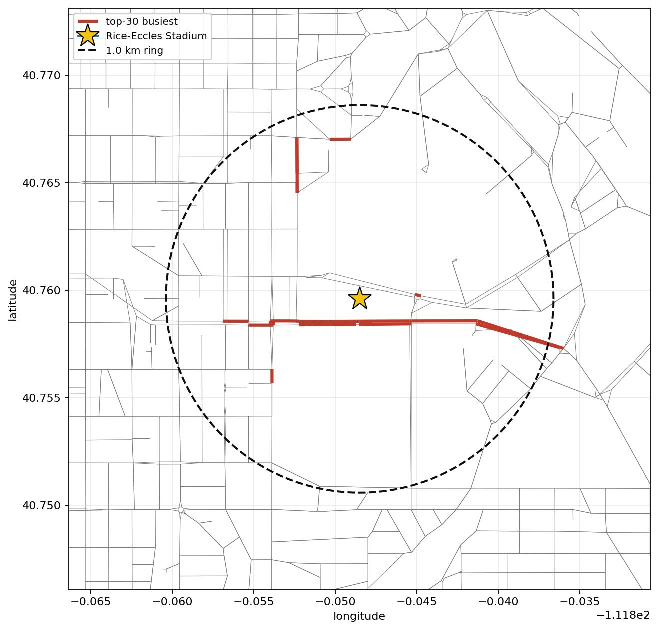
\includegraphics[width=\linewidth]{figures/fig_stadium_corridors_top30.pdf}
\caption{Cluster ranked over $19{:}00$--$19{:}55$ on
Sept 1, 8, and 22.}
\label{fig:stadium-corridors}
\end{figure}

\paragraph{Experimental design.}
The chain's parameters are trained on non-event Saturday pairs at
the same kickoff hour
(Sept~1 $\to$ Sept~8 and Sept~22 $\to$ Sept~29, $19{:}00$--$19{:}55$)
and then frozen. At test time the frozen chain is given the
\emph{trip-origins distribution} of Sept~15, the per-link
per-bin count of trips that start on each link during the
kickoff hour, normalized to a probability. The origins vector
carries the event signal (extra starts around the stadium)
without leaking the link-popularity values we are predicting.
Parameters never see Sept~15 link densities. The output of the
frozen chain on the Sept~15 origins input is compared against
Sept~15 link popularity on the top-$k$ cluster; lower is better.
Both single-phase and two-phase chains are tuned with the same
L-BFGS-B protocol on the training pairs (five multi-start
initializations, $p, \beta, \rho \in [0.01, 0.15]$,
$\alpha_s, \alpha_l$ unbounded).

\paragraph{Headline result: held-out comparison.}
\Cref{tab:heldout-headline} reports the held-out d2m on the
Sept~15 cluster for the proposed two-phase chain, the
single-phase one-stage Markov chain baseline, and three simpler
predictors that drop one component of the pipeline.

\begin{table}[H]
\centering
\caption{Held-out forecast d2m on the Sept~15 stadium cluster.
Parameters fit only on the non-event Saturday pairs (Sept~1
$\to$ Sept~8 and Sept~22 $\to$ Sept~29 at the kickoff hour) and
frozen before evaluation on Sept~15. Test input is the Sept~15
trip-origins distribution after $\gamma$-diffusion. Lower is
better. Read each cell as ``this predictor's mean per-link
relative error, averaged over the $12$ kickoff-hour bins and
the top-$k$ stadium links.''}
\label{tab:heldout-headline}
\resizebox{\linewidth}{!}{%
\begin{tabular}{lcccl}
\toprule
predictor & top-10 & top-20 & top-30 & notes \\
\midrule
two-phase, tuned (ours)   & $\mathbf{0.678}$ & $\mathbf{0.751}$ & $\mathbf{0.848}$ & main method \\
single-phase, tuned       & $0.709$ & $0.826$ & $0.852$ & 1-stage Markov chain \\
two-phase, no dangling fix (v1) & $1.734$ & $2.160$ & $2.054$ & earlier two-phase variant \\
two-phase, no $\gamma$-smoothing & $1.785$ & $2.249$ & $2.084$ & raw Laplace prior \\
$d2d$ (last week's popularity, no chain) & $7.088$ & $8.918$ & $8.062$ & naive baseline \\
\bottomrule
\end{tabular}}
\end{table}

\paragraph{Reading the table.}
The two-phase chain is the best predictor on every cluster
under the held-out protocol, by $0.031$ d2m on top-$10$,
$0.075$ d2m on top-$20$, and $0.004$ d2m on top-$30$ relative
to the single-phase chain. The remaining baselines tell a
consistent story: the naive $d2d$ row uses last week's
popularity and lands at the event-day noise floor; the v1
chain without the dangling-link fix and the no-$\gamma$-smoothing
variant both sit well above the tuned chains, showing that the
dangling correction and the $\gamma$-smoothing component each
earn their place in the pipeline.

\begin{table}[H]
\centering
\caption{Frozen-tuned parameter values per cluster, fit on the
non-event Saturday training pairs (origins $\to$ popularity).
Parameter ranges: $p, \beta, \rho \in [0.01, 0.15]$,
$\alpha_s, \alpha_l$ unbounded. Read each row as ``on this
cluster size, L-BFGS-B converged to these parameters and
produced the d2m bolded in \cref{tab:heldout-headline};
$\alpha_s, \alpha_l$ are unbounded exponents and can fall
outside $[-1, 1]$.''}
\label{tab:event-topk-params}
\resizebox{\linewidth}{!}{%
\begin{tabular}{lcccc|cccc}
\toprule
& \multicolumn{3}{c}{single-phase} & & \multicolumn{4}{c}{two-phase} \\
\cmidrule(lr){2-4}\cmidrule(lr){6-9}
cluster & $p$ & $\alpha_s$ & $\alpha_l$ &
        & $\alpha_s$ & $\alpha_l$ & $\beta$ & $\rho$ \\
\midrule
top-10 & $0.01$ & $-2.39$ &  $+4.67$ &
       & $+3.62$  & $-4.22$  & $0.15$ & $0.01$ \\
top-20 & $0.01$ & $-4.11$ &  $-0.62$ &
       & $-6.43$  & $-1.03$  & $0.01$ & $0.1049$ \\
top-30 & $0.01$ & $+47.36$ & $-15.03$ &
       & $+77.20$ & $-33.47$ & $0.01$ & $0.01$ \\
\bottomrule
\end{tabular}}
\end{table}

\section{Discussion and limitations}
\label{sec:discussion}

\paragraph{What the held-out experiment shows.}
Under proper held-out conditions the two-phase chain remains
the best predictor on the Sept~15 stadium cluster across the
predictors we considered: it beats the single-phase chain, the
v1 two-phase chain without the dangling-node fix, the
no-$\gamma$-smoothing variant, and the no-chain baselines. The
gap between the two-phase chain and the single-phase chain is
smaller than under the in-sample protocol because the
held-out setup denies both chains direct access to the event-day
ground truth, but the ordering is preserved across all three
cluster sizes (top-$10$, top-$20$, top-$30$). Every component
of the pipeline (Laplace pseudo-count, $\gamma = 0.20$
diffusion, dangling-node correction, two-phase split) is shown
to earn its place by an ablation against the corresponding
simpler variant in \cref{tab:heldout-headline}.

\paragraph{Limitations.}
The probe corpus is a biased sample (\cref{sec:counting}): it
oversamples freeway corridors and undersamples residential
streets. The chain therefore predicts \emph{probe-population
link popularity}, not a uniform-vehicle volume. The validation
also tests prediction at a single time scale ($5$-minute bins)
and a single city; cross-city transfer and finer-grained
resolutions are outside scope. Finally, the intervention case
study uses a single known event; an evaluation across many
labeled events would strengthen the generalization claim.

\section{Conclusion}

We presented a two-phase {PageRank} chain that turns a smoothed
per-link popularity prior into a per-link traffic prediction on
a $99{,}716$-link city graph, with all calibration steps
($\sigma$ for map-matching, $\gamma$ for diffusion smoothing,
$\beta$ and $\rho$ for the chain) driven by the data. Under a
proper held-out protocol on a real event (Utah vs Washington,
Sept~15 2018), the two-phase chain beats the single-phase
baseline and a suite of simpler comparators on every stadium
cluster size, validating both the two-phase architecture and
the calibration pipeline.

\begin{thebibliography}{99}

\bibitem{meert2018hmm}
Wannes Meert and Mathias Verbeke.
\newblock HMM with non-emitting states for map matching.
\newblock In \emph{European Conference on Data Analysis (ECDA)}, Paderborn, Germany, July 2018.

\bibitem{leuvenmapmatching}
Wannes Meert.
\newblock \emph{Leuven Map-Matching: a Python library for matching GPS trajectories to road networks}.
\newblock KU Leuven, DTAI Research Group, 2015--2024.
\newblock \url{https://github.com/wannesm/LeuvenMapMatching}.

\bibitem{newson2009hmm}
Paul Newson and John Krumm.
\newblock Hidden Markov map matching through noise and sparseness.
\newblock In \emph{Proceedings of the 17th ACM SIGSPATIAL International Conference on Advances in Geographic Information Systems (GIS '09)}, pages 336--343. ACM, 2009.
\newblock \href{https://doi.org/10.1145/1653771.1653818}{doi:10.1145/1653771.1653818}.

\bibitem{sinnott1984haversine}
Roger W. Sinnott.
\newblock Virtues of the Haversine.
\newblock \emph{Sky and Telescope}, 68:158, 1984.
\newblock \url{https://ui.adsabs.harvard.edu/abs/1984S\%26T....68..158S/abstract}.

\bibitem{snyder1987maps}
John P. Snyder.
\newblock \emph{Map Projections: A Working Manual}.
\newblock U.S. Geological Survey Professional Paper 1395, U.S. Government Printing Office, Washington, DC, 1987.
\newblock Chapter~12, ``Equidistant Cylindrical Projection'', pp.~90--91.
\newblock \url{https://pubs.usgs.gov/pp/1395/report.pdf}.

\bibitem{quddus2007mapmatching}
Mohammed A. Quddus, Washington Y. Ochieng, and Robert B. Noland.
\newblock Current map-matching algorithms for transport applications: state-of-the-art and future research directions.
\newblock \emph{Transportation Research Part C: Emerging Technologies}, 15(5):312--328, 2007.
\newblock \href{https://doi.org/10.1016/j.trc.2007.05.002}{doi:10.1016/j.trc.2007.05.002}.

\bibitem{lou2009stmatching}
Yin Lou, Chengyang Zhang, Yu Zheng, Xing Xie, Wei Wang, and Yan Huang.
\newblock Map-matching for low-sampling-rate GPS trajectories.
\newblock In \emph{Proceedings of the 17th ACM SIGSPATIAL International Conference on Advances in Geographic Information Systems (GIS '09)}, pages 352--361. ACM, 2009.
\newblock \href{https://doi.org/10.1145/1653771.1653820}{doi:10.1145/1653771.1653820}.

\bibitem{agryzkov2023nonlocal}
Taras Agryzkov, Leandro Tortosa, and Jos\'e F. Vicent.
\newblock Extending the Adapted PageRank Algorithm centrality model for urban street networks using non-local random walks.
\newblock \emph{Applied Mathematics and Computation}, 447:127531, 2023.
\newblock \href{https://doi.org/10.1016/j.amc.2023.127531}{doi:10.1016/j.amc.2023.127531}.

\bibitem{gonzalez2008mobility}
Marta C. Gonz\'alez, C\'esar A. Hidalgo, and Albert-L\'aszl\'o Barab\'asi.
\newblock Understanding individual human mobility patterns.
\newblock \emph{Nature}, 453:779--782, 2008.
\newblock \href{https://doi.org/10.1038/nature06958}{doi:10.1038/nature06958}.

\bibitem{helbing2001traffic}
Dirk Helbing.
\newblock Traffic and related self-driven many-particle systems.
\newblock \emph{Reviews of Modern Physics}, 73(4):1067--1141, 2001.
\newblock \href{https://doi.org/10.1103/RevModPhys.73.1067}{doi:10.1103/RevModPhys.73.1067}.

\bibitem{iqbal2014odmatrices}
Md.~Shahadat Iqbal, Charisma F. Choudhury, Pu Wang, and Marta C. Gonz\'alez.
\newblock Development of origin-destination matrices using mobile phone call data.
\newblock \emph{Transportation Research Part C: Emerging Technologies}, 40:63--74, 2014.
\newblock \href{https://doi.org/10.1016/j.trc.2014.01.002}{doi:10.1016/j.trc.2014.01.002}.

\bibitem{yang2017odprobe}
Xiangdong Yang, Yang Lu, and Wei Hao.
\newblock Origin-destination estimation using probe vehicle trajectory and link counts.
\newblock \emph{Journal of Advanced Transportation}, 2017:4341532, 2017.
\newblock \href{https://doi.org/10.1155/2017/4341532}{doi:10.1155/2017/4341532}.

\bibitem{wang2012roadusage}
Pu Wang, Timothy Hunter, Alexandre M. Bayen, Katja Schechtner, and Marta C. Gonz\'alez.
\newblock Understanding road usage patterns in urban areas.
\newblock \emph{Scientific Reports}, 2:1001, 2012.
\newblock \href{https://doi.org/10.1038/srep01001}{doi:10.1038/srep01001}.

\bibitem{zheng2015trajectory}
Yu Zheng.
\newblock Trajectory data mining: an overview.
\newblock \emph{ACM Transactions on Intelligent Systems and Technology}, 6(3):29, 2015.
\newblock \href{https://doi.org/10.1145/2743025}{doi:10.1145/2743025}.

\bibitem{yuan2010tdrive}
Jing Yuan, Yu Zheng, Chengyang Zhang, Wenlei Xie, Xing Xie, Guangzhong Sun, and Yan Huang.
\newblock T-drive: driving directions based on taxi trajectories.
\newblock In \emph{Proceedings of the 18th ACM SIGSPATIAL International Conference on Advances in Geographic Information Systems (GIS '10)}, pages 99--108. ACM, 2010.
\newblock \href{https://doi.org/10.1145/1869790.1869807}{doi:10.1145/1869790.1869807}.

\bibitem{li2015percolation}
Daqing Li, Bowen Fu, Yunpeng Wang, Guangquan Lu, Yehiel Berezin, H.~Eugene Stanley, and Shlomo Havlin.
\newblock Percolation transition in dynamical traffic network with evolving critical bottlenecks.
\newblock \emph{Proceedings of the National Academy of Sciences (PNAS)}, 112(3):669--672, 2015.
\newblock \href{https://doi.org/10.1073/pnas.1419185112}{doi:10.1073/pnas.1419185112}.

\bibitem{jenelius2006importance}
Erik Jenelius, Tom Petersen, and Lars-G\"oran Mattsson.
\newblock Importance and exposure in road network vulnerability analysis.
\newblock \emph{Transportation Research Part A: Policy and Practice}, 40(7):537--560, 2006.
\newblock \href{https://doi.org/10.1016/j.tra.2005.11.003}{doi:10.1016/j.tra.2005.11.003}.

\bibitem{latora2005vulnerability}
Vito Latora and Massimo Marchiori.
\newblock Vulnerability and protection of infrastructure networks.
\newblock \emph{Physical Review E}, 71:015103(R), 2005.
\newblock \href{https://doi.org/10.1103/PhysRevE.71.015103}{doi:10.1103/PhysRevE.71.015103}.

\bibitem{shuman2013gsp}
David I. Shuman, Sunil K. Narang, Pascal Frossard, Antonio Ortega, and Pierre Vandergheynst.
\newblock The emerging field of signal processing on graphs: extending high-dimensional data analysis to networks and other irregular domains.
\newblock \emph{IEEE Signal Processing Magazine}, 30(3):83--98, 2013.
\newblock \href{https://doi.org/10.1109/MSP.2012.2235192}{doi:10.1109/MSP.2012.2235192}.

\bibitem{defferrard2016chebnet}
Micha\"el Defferrard, Xavier Bresson, and Pierre Vandergheynst.
\newblock Convolutional neural networks on graphs with fast localized spectral filtering.
\newblock In \emph{Advances in Neural Information Processing Systems (NeurIPS)} 29, pages 3837--3845, 2016.
\newblock \url{https://arxiv.org/abs/1606.09375}.

\bibitem{horni2016matsim}
Andreas Horni, Kai Nagel, and Kay W. Axhausen (editors).
\newblock \emph{The Multi-Agent Transport Simulation MATSim}.
\newblock Ubiquity Press, London, 2016.
\newblock \href{https://doi.org/10.5334/baw}{doi:10.5334/baw}.

\bibitem{balmer2006matsim}
Michael Balmer, Kay W. Axhausen, and Kai Nagel.
\newblock Agent-based demand-modeling framework for large-scale microsimulations.
\newblock \emph{Transportation Research Record: Journal of the Transportation Research Board}, 1985:125--134, 2006.
\newblock \href{https://doi.org/10.1177/0361198106198500114}{doi:10.1177/0361198106198500114}.

\bibitem{wang2017pagerank}
Minjie Wang, Su Yang, Yi Sun, and Jun Gao.
\newblock Discovering urban mobility patterns with PageRank based traffic modeling and prediction.
\newblock \emph{Physica A: Statistical Mechanics and its Applications}, 485:23--34, 2017.
\newblock \href{https://doi.org/10.1016/j.physa.2017.04.155}{doi:10.1016/j.physa.2017.04.155}.

\bibitem{jiang2009ranking}
Bin Jiang.
\newblock Ranking spaces for predicting human movement in an urban environment.
\newblock \emph{International Journal of Geographical Information Science}, 23(7):823--837, 2009.
\newblock \href{https://doi.org/10.1080/13658810802022822}{doi:10.1080/13658810802022822}.

\bibitem{bazzani2010florence}
Armando Bazzani, Bruno Giorgini, Sandro Rambaldi, Riccardo Gallotti, and Luca Giovannini.
\newblock Statistical laws in urban mobility from microscopic GPS data in the area of Florence.
\newblock \emph{Journal of Statistical Mechanics: Theory and Experiment}, 2010(05):P05001, 2010.
\newblock \href{https://doi.org/10.1088/1742-5468/2010/05/P05001}{doi:10.1088/1742-5468/2010/05/P05001}.

\bibitem{liang2013exponential}
Xiao Liang, Jichang Zhao, Li Dong, and Ke Xu.
\newblock Unraveling the origin of exponential law in intra-urban human mobility.
\newblock \emph{Scientific Reports}, 3:2983, 2013.
\newblock \href{https://doi.org/10.1038/srep02983}{doi:10.1038/srep02983}.

\end{thebibliography}



\appendix
\section{Appendix: classical-form two-phase chain}
\label{app:tp-old-form}

\subsection{Definition}

Let $P_{cs}$ be the column-stochastic out-adjacency of the directed road
network (each column of $P_{cs}$ sums to one and represents the
distribution of next-link probabilities out of a given source link), and
let $E_b$ be the diffused popularity prior at the source bin. We build
the $2N \times 2N$ block transition

\begin{equation}
M_{2N} \;=\;
\begin{bmatrix}
(1-\beta)\, P_{cs} & 0 \\[3pt]
\beta\, I          & P_{cs}
\end{bmatrix},
\qquad
E_{2N} \;=\;
\begin{bmatrix} E_b \\[3pt] 0 \end{bmatrix}.
\label{eq:tp-old-block}
\end{equation}

$M_{2N}$ is column-stochastic, acting directly on probability vectors:
from any link in the up phase, a fraction $(1-\beta)$ of its mass follows
the topology within the up phase and a fraction $\beta$ commits to the
same link in the down phase; once in the down phase, mass keeps following
the topology with no internal restart. The chain iterates

\begin{equation}
v^{(k+1)} \;=\; (1-\alpha)\, M_{2N}\, v^{(k)} \;+\; \alpha\, E_{2N},
\label{eq:tp-old-iter}
\end{equation}

where $\alpha \in (0,1)$ is the global teleportation rate. Component-wise:

\begin{align}
v_{up}^{(k+1)}   &= (1-\alpha)(1-\beta)\, P_{cs}\, v_{up}^{(k)} \;+\; \alpha\, E_b, \\
v_{down}^{(k+1)} &= (1-\alpha)\,\beta\, v_{up}^{(k)} \;+\; (1-\alpha)\, P_{cs}\, v_{down}^{(k)}.
\end{align}

Mass lost through dangling nodes (links with no out-edges) is reinjected
through $E_b$ at each step so the total $\|v^{(k)}\|_1 = 1$ is preserved.
The final prediction is $v = v_{up} + v_{down}$.

\subsection{Estimation}

The chain is evaluated and tuned on the same 840 calendar (t, t+7 days)
pairs as the rest of \cref{tab:ladder-tuning}, with the same source and
target taken from the diffused popularity matrix.

 A \emph{tuned} rung fixes $\alpha = 0.15$ and minimizes
Overall MRE by gradient descent over $\beta \in [0.01, 0.15]$ together
with the road-type exponents $\alpha_s, \alpha_l$ (unbounded), in three
modes that mirror the single-phase ladder: lanes-only, speed-only, and
both.
\end{document}
